\documentclass{article}
\usepackage[utf8]{inputenc}
\usepackage{amsmath}
\usepackage{amsfonts}
\usepackage{amsthm}
\usepackage{amssymb}
\usepackage{graphicx}
\graphicspath{ {./imgs/} }
\usepackage[margin=1in]{geometry}
\usepackage{float}
\usepackage{xcolor}
\usepackage{color}
\usepackage{hyperref}
\usepackage{listings}
\hypersetup{
    colorlinks=true, 
    linktoc=all,     
    linkcolor=blue,  
}
\lstset{
  basicstyle=\ttfamily,
  mathescape
}
\newcommand\todo[1]{\textcolor{red}{TODO: {#1}}}

\title{CSC236 Notes}
\author{}
\date{}

\begin{document}

\maketitle

\tableofcontents

\newpage

\section{Functions}
\subsection{Review}
\textbf{Subsets: }A $\subseteq$ B, i.e., $x \in $ A $\implies x \in $ B\\
\textbf{Union: }A $\cup$ B, i.e., the set of elements contained in A or B.\\
\textbf{Intersection: }A $\cap$ B, i.e., the set of elements contained in both A and B.\\
\textbf{Difference: }A $\setminus$ B, i.e., the set of the elements contained in A excluding the intersection A $\cap$ B.\\
\textbf{Power set: } (P(a) = \{B: B $\subseteq$ A \}, i.e., the set containing all the subsets of A.
For example, for $A = \{1, 2, 3\}$, P(A) = \{\{1, 2\}, $\emptyset$, \{1,2,3\}, \{1,3\}, \{2,3\}, \{1\}, \{2\}, \{3\}\}

\subsection{Functions}
For the function $f : A \rightarrow B$, we say that A is the domain (the set of all possible inputs), B is the codomain (the set of possible outputs), and $f$ is a function from A to B.\\
Everything in A gets mapped to B, but not everything in B needs to be mapped.\\
Each item in the domain must map to at most one item, and all items in the domain must map to something in the codomain. If we want our items in the domain to map to multiple items or to no items, we can change our codomain to be a powerset of possible items, instead.\\
It is also important to specify the domain and codomain when defining a function.
\\
\\
\textbf{Injective functions: }A function $f: A \rightarrow B$ is injective if and only if:
$$\forall x, y \in A, (x \neq y \implies f(x) \neq f(y))$$
In other words, if the inputs are different, then the outputs must be different.\\
By contrapositive, we say: $\forall x, y \in A, (f(x) = f(y) \implies x = y)$.\\
\\
\textbf{The Pigeonhole Principle}\\
Theorem. Let A, B be sets where $\mid$A$\mid$ = $m$, and $\mid$B$\mid$ = $n$, where $m > n$. Then, there is no injective function $f: A \rightarrow B$.\\
In other words, if there are $m$ pigeons, and $n$ pigeonholes, no matter how we assign pigeons to pigeonholes, at least one pigeonhole will have at least $\lceil \frac{m}{n} \rceil$ pigeons. ($\lceil x\rceil$ rounds x up to the nearest integer).\\
\\
\\
\textbf{Injectivity Proofs}\\
Let $f(x) = \begin{cases}
2i & x = a_i\\
2i + 1 & x = b_i
\end{cases}$\\
Prove that the function is injective.\\
\\
Proof. Let x, y be customers s.t. $x \neq y$. We will show that $f(x) \neq f(y)$. We have the following cases:
\begin{enumerate}
    \item Suppose $x$ and $y$ are on different busses. WLOG, assume that $x$ was on the first and $y$ on the second. The, $f(x) \neq f(y)$ since $f(x)$ is even, and $f(y)$ odd.
    \item If $x$ and $y$ were both on the first bus, since $x \neq y$, $x = a_i$ and $y = a_j$ for some $i \neq j$. Thus $2i \neq 2j$, and $f(x) \neq f(y)$ as required.
    \item The case where $x$ and $y$ both on the second bus similar.
\end{enumerate}
\\
\\
\\
\textbf{Surjective Functions: } A function $f: A \rightarrow B$ is surjective if and only if:
$$\forall b \in B, \exists a \in A, (f(a) = b)$$
In other words, everything in the function's codomain must be hit.
\\
\\
\\
\textbf{Bijective Functions: } A function $f: A \rightarrow B$ if and only if it is both surjective and injective.\\
\\
\textbf{Bijectivity Proofs}\\
Let $f(x) = \frac{x}{2}$. Prove it is bijective.\\
Proof. To prove $f(x)$ is bijective, we prove both injectivity and surjectivity.
\begin{enumerate}
    \item Injective. Let $a, b \in \mathbb{R}$, and assume $f(a) = f(b)$. By the definition of $f$, this implies that $\frac{a}{2} = \frac{b}{2}$, which implies $a = b$. Hence, $f$ is injective.
    \item Let $b \in \mathbb{R}$. To show $f$ is surjective, we need to find some number $a \in \mathbb{R}$ such that $f(a) = b$.\\
    We claim $a = 2b$, so we have $f(a) = f(2b) = \frac{2b}{2} = b$. Hence, $f$ is surjective.
\end{enumerate}
$f(x)$ is both injective and surjective, and thus it is bijective.

\subsection{Cantor's Theorem}
\textit{Theorem.} For any set A, there is no surjection between A and $P(A)$.\\
\\
For example, for the set $A = \{1, 2, 3\}$, $P(A) = \{\emptyset, \{1\}, \{2\}, \{3\}, \{1, 2\}, \{1,3\}, \{2, 3\}, \{1,2,3\}\}$, there is no surjective function from the smaller set $A$ to $P(A)$. That is, there is an element in the codomain such that an element in the domain does not hit that element of the codomain.\\
This is true for all finite sets.\\
Imagine $f(x)$ as a function that maps $A$ to $P(A)$. We would get the following table:
\begin{center}
    \begin{tabular}{c|c|c|c}
              & 1 & 2  & 3 \\
\hline
         f(1) & T & F & F\\
         f(2) & F & F & T\\
         f(3) & T & F & T
    \end{tabular}
\end{center}
For the item $1 \in A$, $f(1)$, it maps to the first item in the powerset $P(A)$, $\{1\}$. This continues for all other elements of A.\\
Look at the diagonal (the set D) across the above table, and reverse the signs of them (T becomes F, vice versa). So, we get:
\begin{center}
    \begin{tabular}{c|c|c|c}
              & 1 & 2  & 3 \\
\hline
         f(1) & F & F & F\\
         f(2) & F & T & T\\
         f(3) & T & F & F
    \end{tabular}
\end{center}
Now, we let our set $D = \{2\}$ and the function is considered non-surjective.\\
In other words, $D = \{a \in A: a \not\in f(a)\}$.\\For all possible functions, this procedure must be possible and the grid must work.\\
\\
\begin{proof}
 Let $f: A \rightarrow P(A)$. Let $D = \{a \in A: a \not\in f(a)\}$, and note that $D \subseteq A$. This implies that $D \in P(A)$. To prove that $f$ is not surjective, we show that there is no $a \in A$ such that $f(a) = D$ (D is the subset of the codomain that is not being hit).\\
By contradiction, assume that $D = f(a)$ for some $a \in D$. There are two possible cases, $a \in D$
, or $a \not\in D$.\\
\begin{enumerate}
    \item If $a \in D$, then $a \not\in f(a)$ by the definition of D. However, $f(a) = D$, so $a \not\in D$. This is a contradiction.
    \item If $a \not\in D$, then $a \in f(a)$ but $f(a) = D$ by assumption, so $a \in D$. Contradiction.
\end{enumerate}
In both cases there is a contradiction, so $f$ is not surjective.
\end{proof}
\\
\\
\textbf{Programs and Cantor's Theorem}\\
Let Strings be the set of all possible strings. For each subset A $\subseteq$ Strings (where each A $\in$ P(Strings)), determine whether or not a given input is in A or not in A.\\
As an example, let A = $\{ w \in $ Strings : $w$ is a palindrome\}.\\
Let the set Problems = P(Strings).\\
We say that program P solves a problem A $\subseteq$ Strings if $\forall w \in $ Strings:
$w \in$ A $\iff$ P run on input $w$ prints 1, and nothing else.\\
Identify each program with its source code (a string), so that Programs $\subseteq$ Strings.\\
\\
\textbf{Solution}\\
Let Solves: Programs $\rightarrow$ P(Strings) be the function that maps each program to the program it solves. Each program solves at most one problem, so it is well defined. Determine whether or not Solves is surjective or not.\\
\\
\textbf{Proof: }Computers can not solve all problems, since Solves is not surjective.\\
By contradiction, assume that Solves: Programs $\rightarrow$ P(Strings) is surjective. We want to construct a surjective function from Strings $\rightarrow$ P(Strings), which contradicts Cantor's Theorem.\\
Let $f: $Strings $\rightarrow$ P(Strings) be defined as follows:
$$f(w) = \begin{cases}
Solves(w) & w \in \text{Programs}\\
\emptyset & \text{else}
\end{cases}$$
We claim that $f$ is surjective. Let $b \in$ P(Strings). Since Solves is surjective, then there exists some $a \in$ Programs such that Solves(a) = $b$.\\
Since Programs $\subseteq$ Strings, $a \in$ Strings. By definition of $f$, $f(a) = $Solves(a) $= b$.\\
Thus, $f$ is surjective, contradicting Cantor's Theorem.\\
Therefore, Solves is not surjective.
\\
\section{Binary Relations}
A \textbf{Binary Relation} $R$ over a set $A$ is a way to compare signs of elements of $A$. For any elements $a, b \in A$.\\
If $a$ relates to $b$ under $R$, we write $aRb$.\\
If $a$ does not relate to $b$, we write $a \not{R}b$
\subsection{Properties of $<$}
Example: What are some properties of $<$ on $\mathbb{N}$?\\
\begin{enumerate}
    \item \textbf{Irreflexive: } $\forall x \in \mathbb{N}, x \not < x$ \ | \ $\forall a \in A, a \not R a$\\
    In other words, there are no self loops.\\
    \item\textbf{Asymmetric: } $\forall,b \in \mathbb{N},a < b \implies b \not < a \ | \ \forall a,b \in A, aRb \implies b \not R a $\\
    In other words, if $a$ goes one way, then $b$ is not going that way.\\
    Note that asymmetric implies irreflexive.
    \item \textbf{Transitive: }$\forall a,b,c, a < b \land b < c \implies a < c$ \ | \ $\forall a,b, c \in \mathbb{N}, aRb \land bRc \implies aRc$. \\
    \item \textbf{Connected: } $\forall a,b, a\neq b \implies a < b \lor b > a \ | \ \forall a,b \in A, a \neq b \implies aRb \lor bRa$\\
\end{enumerate}
\subsubsection{Strict Orders}
Let $R$ be a relation over a set $A$. $R$ is \textbf{strict (partial) order} if it is:
\begin{enumerate}
    \item reflexive,
    \item asymmetric,
    \item and transitive
\end{enumerate}
If $R$ is also connected, then $R$ is a \textbf{strict total order}.\\
\\
Intuitively, if $R$ is a strict total order, we think of it as being like $<$ or $\prec$.\\
If $R$ is a strict partial order, we think of it as being like $<$ or $\prec$, but some elements may not be comparable.\\
\\
\underline{Examples of Strict Total Order: }Dictionary orders\\
\underline{Examples of Strict Partial Order: }Prerequisites/Dependencies, Little-O, IsDescendantOf, $\subsetneq$
\subsection{Hasse Diagrams}
Since we know that a relation can be transitive, edges are oftentimes redundant. Therefore, we only need to draw edges between $a, b$ if $aRb$ and there is no $c$ for which $aRc \land cRb$.\\
\\
Formally, for any strict order $R$ over a set $A$, the \textbf{Hasse Diagram} of $R$ has an edge from $a \to b \iff aRb$ and there does not exist $c \in A : aRc \land cRb$. 
\subsubsection{Irreflexive and Transitive Implies Asymmetric}
Theorem. Let $R$ be a binary relation over a set $A$. If $R$ is irreflexive and transitive, then it is asymmetric.\\
\begin{proof}
    Let $a,b \in A : aRb$. We WTS $b\not{R}A$. By contradiction, assume $bRa$.\\
    \\
    Since $aRb, bRa$ and $R$ is transitive, we have $aRa$. However this contradicts the fact that $R$ is irreflexive (since it's self loop). Therefore, $R$ is asymmetric.\\
\end{proof}
\\
\\
\subsubsection{New Definition of Strict Orders}
Knowing that irreflexive and transitive implies asymmetric, we can rewrite our definition of strict orders.\\\\
Let $R$ be a relation over a set $A$. $R$ is a \textbf{strict partial order} if it is irreflexive and transitive.\\
If $R$ is also connected, then $R$ is a \textbf{strict total order}.

\subsection{Non-Strict Partial Orders}
\subsubsection{Antisymmetric}
A binary relation $R$ over a set $A$ is called \textbf{antisymmetric} is 
$$\forall a,b \in A (aRb \land bRa \implies a = b)$$
Contrapositive: $\forall a,b \in A (a \neq b \implies a\not R b \lor b\not R a)$

\subsubsection{Partial Orders}
A binary relation is called a \textbf{partial order} if it is:
\begin{enumerate}
    \item reflexive,
    \item antisymmetric,
    \item transitive
\end{enumerate}
A binary relation is called a \textbf{total order} if it is a partial order and connected.
\subsection{Properties of SameX}
\begin{enumerate}
    \item \textbf{Transitive: }$\forall a,b,c, a < b \land b < c \implies a < c$ \ | \ $\forall a,b, c \in \mathbb{N}, aRb \land bRC \implies aRc$
    \item \textbf{Reflexive: }$\forall a \in A, aRa$\\
    Intuitively, if every element relates to itself then it is reflexive.
    \item \textbf{Symmetric: }$\forall a,b \in A, aRb \implies bRa$\\
    Intuitively, if every edge is bidirectional (goes both ways), then it is symmetric.
\end{enumerate}
\subsubsection{Equivalence Relations}
Equivalence relations are:
\begin{enumerate}
    \item reflexive,
    \item transitive,
    \item and symmetric
\end{enumerate}
Intuition: If R is an equivalence relation and $aRb$, $a$ is in some way ``equivalent'' to $b$.
\\
\\
\underline{Examples:}
\begin{enumerate}
    \item =
    \item $\equiv_3$ is defined on $\mathbb{N}$ where for $a,b \in \mathbb{N},$\\
    $a \equiv_3 b \iff \exists k \in \mathbb{Z} : (a = b + 3k)$ \ (i.e., $a = b$ (mod 3)
    \item SameNumberOfVertices defined on the set of polygons.
    \item $\Theta$
\end{enumerate}

\subsubsection{Example Proof of Equivalence Relations}
We want to show $a \equiv_3 b \iff \exists k \in \mathbb{Z} : (a = b + 3k)$ \ (i.e., $a = b$ (mod 3).\\
To prove, we must show it is reflexive, symmetric, and transitive.
\begin{proof}
\textbf{Reflexive: }Let $a \in \mathbb{N}$, then $a = a + 3 \cdot 0$. Hence, $a \equiv_3 a$.\\
\\
\textbf{Symmetric: }Let $a, b \in \mathbb{N}$, and suppose $a \equiv b$ (mod 3). Then, there is some $k \in \mathbb{Z}$ such that $a = b + 3k$.\\
By rearranging, we get $b = a + 3(-k)$. Hence, $b \equiv_3 a$.\\
\\
\textbf{Transitive: }Let $a,b,c \in \mathbb{N}$ and suppose $a \equiv_3 b$ and $b \equiv_3 c$. Then, there exists $k_1, k_2 \in \mathbb{Z}$ such that $a = b + 3k_1$ and $b = c + 3k_2$. Substituting the second equation into the first we get:
\begin{align*}
    a & = c + 3k_2 + 3k_1\\
    & = c + 3(k_2 + k_1)
\end{align*}
Thus, there exists a $k = k_2 + k_1$ such that $a = c + 3k$. Thus, $a \equiv_3 c$. 
\end{proof}

\subsubsection{Equivalence Classes}
Let $R$ be an equivalence relation on a set A. For any $a \in A$, define the \textbf{equivalence class of a with respect to R}, denoted $[a]_R$, to be the set of elements that relate to it, i.e.,
$$[a]_R = \{b \in A: aRb \}$$

\subsubsection{Partitions}
Let $A$ be any set. Let $X$ be a set of subsets of A (i.e., $X \subseteq P(A))$.\\
X is a \textbf{partition} of A if for every $a \in A$, $a$ is in exactly one element of $X$.

\subsubsection{Equivalence Classes and Partitions}
Theorem. Let R be an equivalence relation on a set A. Then, the set of equivalence classes of R is a partition of A. That is, every element of $A$ is in exactly one equivalence class.
\\\\
Lemma. For any $a, b \in A$, $[a]_R = [b]_R \iff aRb$
\begin{proof}
For the forward direction assume $[a]_R = [b]_R$. Since R is an equivalence relation, R is reflexive. Thus bRb, and $b \in [b]_R$. Since $[a]_R = [b]_R, b ] \in [a]_R$. By definition of $[a]_R$, it must be the case that $aRb$.\\
\\
For the backward direction, assume $aRb$. We'll show $[b]_R \subseteq [a]_R.$ Let $x \in [b]_R$, then we have $bRx$. Next, since $aRb$ and $bRx$, by transitivity, $aRx$, and hence $x \in [a]_R$.\\
\\
Now, we show $[a]_R \subseteq [b]_R$. Note that since R is symmetric and $aRb$,  we also have $bRa$. Let $x \in [a]_R$. Then we have $aRx$. Since $bRa$ and $aRx$, by transitivity, $bRx$ and hence $x \in [b]_R$.\\
Finally, since $[a]_R \subseteq [b]_R$ and $[b]_R \subseteq [a]_R$, $[a]_R = [b]_R$ as required.
\\
So, $[a]_R \subseteq [b]_R \land [b]_R \subseteq [a]_R \implies [a]_R = [b]_R$.\\
\end{proof}
We can use our lemma to prove that the set of equivalence classes forms a partition.
\begin{proof}
Let R be an equivalence relation over a set A. We WTS that every element of A is in precisely one equivalence class.\\
Let $a \in A$, since R is reflexive, $aRa$ and hence $a \in [a]_R$. Thus $a$ is in at least one equivalence class.\\
\\
By contradiction, suppose $a$ was also in another equivalence class $[b]_R$ such that $[a]_R \neq [b]_R$. Since $a \in [b]_R, bRa$. By the backwards direction of the lemma, we have $[b]_R = [a]_R$, which is a contradiction.\\
\end{proof}

\section{Graphs}
A \textbf{graph} $G = (V, E)$ is a pair of sets $(V,E)$ where $V$ is a set of vertices and $E$ is a set of pairs of edges.\\
If $E$ is a set of unordered pairs, the graph is \texbf{undirected}, and if $E$ is a set of ordered pairs, the graph is \textbf{directed}.
\begin{enumerate}
    \item Undirected sets are denoted as a set of sets (i.e., $E = \{ \{a,b\}, \{b, c\} \}$)
    \item Directed sets are denoted as a set of tuples (i.e., $E = \{ (a, b), (b, c) \}$
\end{enumerate}
\\
\textbf{Examples of Graphs: } Wifi networks, book reviews, genetic trees, courses and prerequisites, vector graphics, map locations, contact tracing, social media networks, web links, tournament brackets, binary relations, functions.

\subsubsection{Weights}
Sometimes edges can have an associated weight. Formally, we define a function $w: E \to \mathbb{R}$ where $w ( \{u, v\})$ is the weight of the edge $\{u, v\}$.

\subsection{Matching}
Let $G = (V, E) $ be a graph. A matching $M \subseteq E$ is a subset of edges that do not share any endpoints (i.e., every vertex appears in at most one edge in $M$.\\
\\
A matching is \textbf{perfect} if every vertex appears exactly once in the matching.\\
If each of the edges has a weight, then the weight of a matching is the sum of the weights of edges in $M$.

\subsubsection{Matching Problem}
\textbf{Input: }A graph $G = (V, E)$\\
\textbf{Output: }A matching $M \subseteq E$.\\
Usually, we want $|M|$ to be as large as possible. Sometimes, we want to maximize/minimize the weight of the matching as well.

\subsubsection{Matchings in the Real World}
You want to match students that are compatible with one another, but also want to match as many students as possible together.\\
So, we analyze:
\begin{enumerate}
    \item What are the vertices of the graph?
    \item What are the edges of the graph?
    \item What are the edge weights?
    \item What properties of the graph are desired?
\end{enumerate}
For this scenario, our vertices are the students, the edges are from each student to another, the edge weights are their compatibility, and we want to match as many students as possible that have high weights.

\subsection{Paths}
\textbf{Adjacent - } Two vertices $u, v \in V$ are adjacent if $\{u, v\} \in E$.
\\
\\
A sequence of distinct vertices $(v_1, ..., v_n)$ is a \textbf{path} from $v_1$ to $v_n$ if for every $i \in \{1, ..., n - 1\}$, $v_i$ and $v_{i + 1}$ are adjacent.\\
The \textbf{length} of the path is the number of edges in the path.
\subsubsection{Path Finding Problem}
\textbf{Input: }A graph $G = (V, E)$, and two vertices $u, v \in V$.\\
\textbf{Output: }A path from $u$ to $v$ in $G$, i.e., a sequence of vertices $(v_1, v_2, ..., v_n)$ where $v_1 = u$ and $v_n = v$.\\
Typically, we want to find the the shortest path possible for the graph. If each edge has a weight, we may also want to find the path with the smallest total weight.
\subsubsection{Example of Path Finding}
Start at a random Wikipedia page, and try to find a specific article (i.e., University of Toronto).
\\
Our vertices are the set of wikipedia articles,\\ 
our edges are the direct edges from one wikipedia article to another, and we want the path $a$ with the shortest number of edges from one vertex to another.\\

\subsection{Cycles}
Let $G = (V, E)$ be an undirected graph.
A sequence of vertices $(v_1, ..., v_n)$ is a \textbf{cycle} if $(v_1, ..., v_n)$ is a path, $v_1 = v_n$ and $\{v_{n - 1} - v_n\} \in E$.\\
\\
A cycle is called \textbf{Hamiltonian} if every vertex appears in the cycle exactly once (except for the start/end vertex, which appears twice).\\
A Hamiltonian cycle is a permutation of the vertices, but must keep in that the edges must exist.
\\
\subsubsection{Cycle Problem}
\textbf{Input: }A graph $G = (V, E)$ and a starting vertex $h$.\\
\textbf{Output: }A Hamiltonian cycle in $G$ starting with $h$ that minimizes the total edge weights.
\subsubsection{Example of Cycle Problem}
You are a traveling salesperson and want to travel to every house possible.\\
When we consider the weight, we want to find the cycle path that has the smallest total weight.

\subsection{Coloring}
Let $G = (V, E)$ be a graph and let $C$ be a set of $k$ colours.\\
A $k-$(vertex) colouring of $G$ is a function $f: V \to C$ where for any pair of adjacent vertices $u, v$ (any edge $\{u, v\} \in E$), we have:
$$f(u) \neq f(v)$$
Think of $f$ as assigning vertices to colours. A $k$ colouring is a way to assign each vertex one of $k$ colours such that adjacent vertices have different colours.
\\
\\
\textbf{Examples of Colouring: }Sudoku, Fill puzzles.
\subsubsection{Colouring Problems}
\textbf{Input: }A graph $G = (V,E)$, and a number $k \in \mathbb{N}$.\\
\textbf{Output: }A $k$-colouring of $G$.\\
\\
Sometimes, you're also given a partial colouring and asked to complete it to a full colouring. This is called \textbf{precolouring extension}.

\subsection{Independent Sets}
Let $G = (V, E)$ be a graph. A subset of vertices is $I \subseteq V$ is called an \texbf{independent set} if none of the vertices in $I$ are adjacent.\\
For example, for all $u,v \in I, \{u, v\} \not\in E$.

\subsubsection{Modelling Independent Set Problems}
\textbf{Input: }A graph $G = (V,E)$ a number $k \in \mathbb{N}$ with $k > 1$.\\
\textbf{Output: }An independent set $I \subseteq V$ in $G$ of size $k$.\\
\\
Sometimes, we don't give a number $k$ and ask for the largest possible independent set instead.

\subsection{Other Problems with Graphs}
There are many more problems on graphs that are good to know (you can see some of them on the documentation for networkx).
For example, centrality, chains, dominance, planarity, etc. all deal with graphs and various properties/problems involving graphs.\\
\\
We can often convert one problem into another in Computer Science. If problem $A$ can be converted to problem $B$, then $A$ \textbf{reduces} to $B$. This idea is how one defines a partial order on the set of problems in terms of their difficulty.\\
For example, if $A$ reduces to $B$, then $A$ is at most as hard as $B$ (since if we solve $B$, then we can solve $A$).

\subsection{Trees}
Let $G = (V, E)$ be any graph.
\begin{enumerate}
    \item $G$ is \textbf{connected} if for every pair of distinct vertices $u, v$ there is a path from $u$ to $v$.
    \item $G$ is \textbf{acyclic} if there are no cycles in $G$.
\end{enumerate}
A graph is considered a tree if it is connected and acyclic.\\
\\
Generally, if a graph has more edges, then it is more likely to be connected but also be a cycle.\\
If a graph has fewer edges, it is more likely acyclic, but less likely to be connected.\\
\\
Trees are considered to have an `ideal' number of edges. Therefore, trees are considered \textbf{minimally connected graphs}, meaning it is connected but removing an edge causes the tree to be disconnected.\\
\\
Trees are \textbf{maximally acyclic graphs}, meaning that it is not cyclic, but adding any edge creates a cycle.\\
\\
Note that:
\begin{center}
    Tree $\iff$ Minimally Connected $\iff$ Maximally Acyclic
\end{center}
\\
A \textbf{binary tree} is a tree with at most 2 "children", or 3 edges between one vertex.
\subsubsection{Proof of Minimally Connected}
\begin{proof}
Let $G$ be a tree. We WTS that removing any edge causes the tree to be disconnected.\\
Let $\{u, v\}$ be an edge in $G$. By contradiction, assume that we can remove $\{u, v\}$ and still be connected. Then, there must be a path $(u = x_1, ..., x_n)$ from $u \to v$ that does not use $\{u, v\}$. Then $(x_1 = u, ..., x_n = v, x_1 = a)$, which is a contradiction.
\end{proof}

\subsubsection{Proof of Maximally Acyclic}
\begin{proof}
Let $G$ be a tree. We WTS that adding any edge creates a graph.\\
Let $\{u,v\}$ be any edge not in $G$. Let $G' = G$ with $\{u,v\}$ added.\\
By contradiction, assume $G'$ is still acyclic.
This implies $G'$ is acyclic and connected (since adding an edge doesn't destroy connectivity), implying that $G'$ is still a tree.\\
By the previous theorem, $G'$ is minimally connected, so removing any edge from $G'$ disconnects the graph. When we remove that same edge, we get the graph $G$ back. However, this implies $G$ is not connected, which is a contradiction.
\end{proof}\\
\\
\textbf{Alternate Proof}
\begin{proof}
Let $G$ be a tree. We WTS that adding any edge makes it cyclic.\\
Let $\{u,v\}$ be any edge not already in $G$.\\
Since $G$ is connected, there exists a path from $u$ to $v$. $P = (u = x_1, ..., x_n = v)$. Once we add $\{u, v\}$, there is a cycle ($u = x_1, ..., x_n = v, u)$.
\end{proof}
\subsection{Edges and Trees}
The number of edges of a graph is one less the number of vertices. That is:
$$|E| = |V| - 1$$
\section{Induction}
Induction is used to prove statements of the following form:
$$\forall n \in \mathbb{N} (P(n))$$
Note that $P$ is a predicate for the natural numbers, being true or false for any natural number $n$,\\
Induction is super useful when analyzing the correctness and runtime of algorithms.\\
Formally, we write:
$$( P(0) \land \forall k \in \mathbb{N}. (P(k)) \implies P(k + 1))) \implies \forall n \in \mathbb{N}. P(n))$$
It is sufficient to prove for any induction proof:
\begin{enumerate}
    \item Base Case (usually the smallest number that works, or P(0)).
    \item Inductive step (assume $P(k)$ is correct (inductive hypothesis), then show $P(k + 1)$ is correct.
\end{enumerate}
\subsection{Binary Trees}
Binary trees are binary if they have 0, 1, or 2 vertices.\\
They are called perfect binary trees if all the leaves are at the same level, and each vertex has exactly two children.\\
\\
The number of vertices in a perfect binary tree for a tree of height $n$ (starting at $n = 0$) is $2^{n + 1} - 1$.
\begin{proof}
We want to show $\forall n \in \mathbb{N}.2^{n + 1} - 1$.\\
Base case: $n = 0$\\
$2^0 = 1 = 2^0 + 1 - 1$, which holds.\\
\\
Inductive step: Let $ k \in \mathbb{N}$ be any natural number, and assume that $2^{k + 1} - 1$ holds.\\
We want to show that $2^{k + 1 + 1} - 1$ holds.
\begin{align*}
    2^0 + 2^1 + ... + 2^k + 2^{k + 1} & = (2^0 + 2^1 + ... + 2^k) + 2^{k + 1}\\
    & = (2^{k + 1} - 1) + 2^{k + 1}
    & = 2^{k + 1 + 1} - 1
\end{align*}
\end{proof}
\subsection{Odd Squares}
We want to show $\forall n \in \mathbb{N}, n \geq 1 ( \sum^{n}_{i = 1} 2i - 1 = n^2)$
\begin{proof}
Let $P(n)$ be the predicate: $\sum^{n}_{i = 1} 2i - 1 = n^2$\\
Base Case: P(1)\\
$\sum^{n}_{i = 1} 2i - 1 = 1 = 1^2$, which holds.\\
\\
Induction Step: Let $k \in \mathbb{N}$ be any natural number with $k \geq 1$.\\
Assume $P(k)$ holds, namely $1 + 3 + 5 + ... + 2k - 1 = k^2$.\\
We WTS $P(k + 1)$:
\begin{align*}
    1 + 3 + 5 + ... + 2k - 1 + 2k + 1 & = k^2 + 2k + 1\\
    & = (k + 1)^2
\end{align*}
\end{proof}
\subsection{Divisibility}
We WTS $\forall n \in \mathbb{N}. (n^3 - n + 3)$ is divisible by 3.
\begin{proof}
Let $P(n)$ be the predicate: $n^3 - n + 3 = 3x$ for some $x \in \mathbb{Z}$.\\
Base Case: P(0)\\
$0^3 - 0 + 3 = 3$, where $3(1) = 3$.\\
\\
Inductive Step :Let $k \in \mathbb{N}$. Assume $k^3 - k + 3 = 3x$ for some $x \in \mathbb{Z}$.
\begin{align*}
    (k+1)^3 - (k + 1) + 3 & = k^3 + 3k^2 + 3k + 1 - k - 1 + 3\\
    & = 3x + 3k^2 + 3k + 1  - 1\\
    & = 3(x + k^2 + k)
\end{align*}
\end{proof}
\subsection{Units Digit}
We WTS $\forall n \in \mathbb{N}$, the units digit of $7^n$ is $1, 3, 7, 9$.
\begin{proof}
Base Case: $P(0)$\\
$7^0 = 1$, which is true.
\\
Inductive Step: Let $k \in \mathbb{N}$. Assume $7^k$ holds. We WTS $7^{k + 1}$. There are multiple cases:
\begin{enumerate}
    \item If $7^k$ ends in $1$: $7^{k + 1} = 7^k \cdot 7$: has units digit 7.
    \item If $7^k$ ends in 3, $7^{k + 1}$ ends with 1.
    \item $7 \to 9$
    \item $9 \to 3$
\end{enumerate}
\end{proof}
\subsection{Inequalities}
$\forall n \in \mathbb{N}. (n^2 \leq 2^n)$\\
However, this is not true for $n = 3$:\\
$3^2 = 9 \not{\leq} 2^3 = 8$
\\
\\
Instead, we would have to write: $\forall n \in \mathbb{N}, n \geq 4. (n^2 \leq 2^n)$
\begin{proof}
Base Case: $4^2 = 16 = 2^4$, so $P(4)$ holds.\\
\\
Inductive Step: Let $k \in \mathbb{N}, k \geq 4$. Assume $k^2 \leq 2^k$ is true. We WTS $(k + 1)^2 \leq 2^{k + 1}$.
\begin{align*}
    (k + 1)^2 & \leq 2^{k + 1}\\
    k^2 + 2k + 1 & = 2^k + 2k + 1\\
    & \leq k^2 + (k - 2) \cdot k + 1\\
    & = k^2 + k^2 - 2k + 1\\
    & \leq k^2 + k^2 & \text{Since }-2k + 1 \text{is always negative.}\\
    & = 2k^2 \\
    & \leq 2 \cdot 2^k\\
    & = 2^k + 1
\end{align*}
\end{proof}
\subsection{Same Coloured Birds}
Claim. $\forall n \in \mathbb{N}$, a set of $n$ birds will all have the same colour.\\
This statement is false.\\
\\
Make sure that your inductive step does not assume anything more than what your clam is.
\section{Complete Induction}
Complete induction is another way to prove statements of the form $\forall n \in \mathbb{N}.(P(n))$\\
Instead of our regular inductive step, we instead do:
$$\forall k \in \mathbb{N}.(P(0) \land P(1) \land ... \land P(k)) \implies P(k + 1))$$
In other words:\\
Let $k \in \mathbb{N}$ be an arbitrary natural number, and assume for every $i \in \mathbb{N}$ with $i \leq k, P(i)$ holds. We'll show $P(k + 1)$.\\
\\
Complete inductions have a stronger inductive hypothesis, however proofs are more prone to making mistakes than regular induction proofs.
\subsection{Breaking Chocolate}
Claim. Let $n \in \mathbb{N}, n \geq 1$ be any natural number. A chocolate bar with $n$ individual pieces require $n - 1$ breaks to split the bar into individual pieces.
\begin{proof}
Base Case. For $n = 1$, the chocolate bar is in a single piece, so requires $1 - 1 = 0$ breaks.\\
Inductive Step. Let $k \in \mathbb{N}, k \geq 1$ be an arbitrary natural number at least $1$, and assume $P(i)$ is true for all $i \leq k$. We need to show $P(k + 1)$ is true.\\
Let $B$ be a bar of chocolate with $k + 1$ pieces, and select any way to break the bar. We are left with two blocks of chocolate size $a$ and $b$, where $a+b = k + 1, a \leq k$, and $b \leq k$.\\
Applying the inductive hypothesis to each of these blocks, we have that the two blocks require $a - 1$ and $b - 1$ breaks respectively. Therefore, the total number of breaks (including the initial) is $a + b - 2 + 1 = k$, as required.
\end{proof}
\subsection{Multiple Base Cases}
Claim. For any $n \geq 8,$ there exists $a, b \in \mathbb{N}$ such that $n = 3a + 5b$.
\begin{proof}
Base Cases: Since $8 = 3 + 5, 9 = 3 + 3 + 3, 10 = 5 + 5$, we can make postages of $8,9$, and $10$.\\
Inductive Step: Let $k \geq 10$ and assume for any $8 \leq i \leq k$, we can make a postage of $i$ cents using only $3$ and $5$ cent stamps. We'll show that you can make a $k + 1$ postage.\\
Use one 3 cent stamp, and make a $k - 2$ postage. Since $8 \leq k - 2 \leq k$, the induction hypothesis applies, and we can make $k - 2$ using only 3 cent and 5 cent stamps.\\
So together, we made a $k + 1$ postage.
\end{proof}
We can still write this proof using regular induction, just using multiple cases in the inductive step.
\begin{proof}
Base Case. We can make an 8 cent postage using one 3 cent stamp and one 5 cent stamp.\\
Inductive Step: Let $k \geq 8$ and assume $8 \leq i \leq k$, we can make a postage of $i$ using only 3 and 5 cent stamps.\\
We'll show that you can also make a $k + 1$ postage. Let $a, b$ be such that $k = 3a = 5b$. There are two cases:
\begin{enumerate}
    \item $b \geq 1$: We can create $k + 1$ by removing a 5 cent stamp and adding a 2 3 cent stamp.
    \item $b = 0$: Since $k \geq 8$, $a \geq 3$, and we can create $k + 1$ by removing 3 3 cent stamps and adding 2 5 cent stamps.
\end{enumerate}
\end{proof}
In fact, we don't even prove this using induction.
\begin{proof}
Let $n$ be any postage with $n \geq 8$. In lecture 2, we showed $\equiv_3$ is an equivalence relation with exactly 3 equivalence classes corresponding to $0, 1, 2$ (mod 3).\\
Then, since the equivalence classes partition $\mathbb{N}$, $n \equiv_3 8$, $n \equiv_3 9$ or $n \equiv_3 10$.\\
If $n \equiv_3 8$, then by definition of $\equiv_3$, $n = 8 + 3k$ for some $k \in \mathbb{Z}$. Note that since $n \geq 8$, $k$ is non-negative. since we can also make $n$ by adding $k$ 3 cent stamps.\\
Other cases similar.
\end{proof}

\section{Structural Induction}
Previous induction proofs use the set of natural numbers to prove something ($\forall n \in \mathbb{N}, P(n)$).\\
However, in real life, there are other sets other than the natural numbers (e.g., lists, trees, logical formulas), such as:
$$\forall \text{Trees} T, P(T)$$
For this, we need a more general way for these proofs.

\subsection{Generated By}
\begin{enumerate}
    \item Let $U$ be some set (i.e., $U$ is the universe).
    \item Let $B \subseteq U$ (i.e., the base cases).
    \item Let $F$ be a set of functions, where each function $f \in F$  has a domain $U^m$ and codomain $U$.\\
    $f$ maps a tuple of elements of $U$ to a single element of $U$ (i.e., $F$ is a set of construction operations).
\end{enumerate}
The set \textbf{generated from} $B$ by the functions in $F$ is a set of elements that can be obtained by applying function in $F$ to elements of $B$ a finite number of times.

\subsection{Interpreting the Natural Numbers}
We can define $\mathbb{N}$ as $\{0, 1, 2, ... \}$.\\
Let the function $\AddOne$ be the function that maps $x \to x + 1$.\\
Then, $\mathbb{N}$ is the set that can be reached by applying $\AddOne$ to $\{0\}$ a finite number of times.
\\
Using our formula of generation, we can say $\mathbb{N}$ is:
\begin{enumerate}
    \item $U + \mathbb{R}$
    \item $B = \{0\}$
    \item $F = \{\AddOne\}$
\end{enumerate}
Therefore, $\mathbb{N}$ is the set generated from $B$ by functions in $F$.

\subsection{List[X]}
Let $X$ be some set, and let $\List[X]$ be the set of lists of elements in $X$.\\
For each $x \in X$, let $\Append_x$ be a function that takes in a $I$ and appends $x$ to $I$.
\begin{enumerate}
    \item Let $B = \{[]\}$.
    \item Let $F = \{\Append_x : x \in X\}$
\end{enumerate}
Then, $\List[X]$ is the set generated from $B$ by functions in $F$.

\subsection{Defining Structural Induction}
Let $C$ be a set generated from $B$ by the functions in $F$.\\
If:
\begin{enumerate}
    \item $\forall b \in B, P(b)$
    \item $\forall f \in F$ on $m$ inputs, $\forall a_1, ..., a_m \in C$,
    $$(P(a_1) \land P(a_2) \land ... \land P(a_m)) \implies P(f(a_1, ..., a_m))$$
\end{enumerate}

Then, $\forall x \in C, P(x)$.\\
\\
In English, we say:
Let $P$ be any predicate.
\begin{enumerate}
    \item If $I$ can show $P$ is true for all of the base cases,
    \item and $I$ can show that for every construction function, if $P$ holds for the inputs to the construction function then $P$ must hold for the output of the construction function,
\end{enumerate}
Then, $P$ holds for every element constructed from the base cases and the construction functions.

\subsubsection{Recovering Regular Induction}
$\mathbb{N}$ is generated by $\{0\}$ and $\AddOne$. So, substituting $\mathbb{N}$ for $C$, $\{0\}$ for $B$ and $\{\AddOne\}$ for $F$ in structural induction, we get:
\begin{enumerate}
    \item $\forall b \in \{0\}, P(b)$ (note this is just $P(0)$.
    \item $\forall f \in \{\AddOne\}$ on $m$ inputs, for every $a_1, ..., a_m \in \mathbb{N}$,
    $$P(a_1) \land P(a_2) \land ... \land P(a_m) \implies P(f(a_1, ..., a_m))$$
    (note this is just $\forall k \in \mathbb{N}, P(k) \implies P(k + 1))$
\end{enumerate}
Then, $\forall x \in \mathbb{N}, P(x)$.\\
\\
This generalized formalization of induction shows intuitively why we can change the base cases. We just show $P$ holds for every number in the set $\mathbb{N}_{\geq 4} = \{4,5,6\}$, which is just generated from the set $\{4\}$, and the function $\AddOne$.

\subsection{Perfect Binary Trees Using Structural Induction}
Let $\PerfectBinaryTrees$ be the set of perfect binary trees, and write it as being generated from a set by some function.
\begin{enumerate}
    \item $U$ = Set of all graphs
    \item $B = \{Single node\}$
    \item $\JoinPerfectTrees: U \times U \to U$ maps $(G_1, G_2)$ to the tree with $G_1$ as the left subtree and $G_2$ as the right subtree $\iff$ $G_1$ and $G_2$ are perfect binary trees of the same height.\\
    Otherwise, it maps to the graph with a single node.
\end{enumerate}
Claim. Let $P(G)$ be the predicate that if $G$ is a perfect binary tree of height $h$, then $G$ has $2^{h + 1} - 1$ vertices.
\begin{proof}
The base case is the graph consisting of a single node. It has height $0$ and $2^{0 + 1} - 1 = 1$ vertices. Hence, the base case is true.\\
Inductive Step: Let $G_1 = (V_1, E_1), G_2 = (V_2, E_2)$ be any graphs and assume $P$ holds for $G_1$ and $G_2$. We WTS that $P$ also holds for $\JoinPerfectTrees(G_1, G_2)$.\\
Note that if $G_1$ and $G_2$ are not perfect binary trees of the same height $h$, $\JoinPerfectTrees(G_1, G_2)$ is the single node graph, which is the base case.\\
Otherwise, $G_1$ ad $G_2$ are both perfect binary trees of height $h$. By the induction hypothesis, $|V_1| = |V_2| = 2^{h + 1} - 1$.\\
$\JoinPerfectTrees(G_1, G_2)$ is then a perfect binary tree of height $h + 1$ with:
$$1 + 2(2^{h + 1} - 1) = 2^{h + 2} - 1$$
vertices as required.
\end{proof}

\subsection{Construction Sequences}
Complete induction can be used in place of structural induction.\\
\\
Let $C$ be the set generated from $B$ by the functions in $F$. We define a \textbf{construction sequence} of length $n - 1$, to be q sequence of elements $(x_1, ..., x_n)$ where for each $i \in [n]$, either:
\begin{enumerate}
    \item $x_i \in B$
    \item $x_1 = f(x_{j_1}, ..., x_{j_m}$ for some $f \in F$, and $j_1, ..., j_m < i$.
\end{enumerate}
In other words, every element in a sequence is either in the base set $B$ or is constructed by applying a construction function to earlier elements in the sequence.\\
\\
We can define a $C_i$ that is the set where $x \in C_i$ if there exists some construction sequence of length at most $i$ ending in $x$. Then $C = C_0 \cup C_1 \cup ...$\\
Instead of using structural induction, we can do induction on the length of the construction sequences of at most $k$, then $P$ also holds for elements with construction sequences of length at most $k + 1$.\\
Usually, the length of construction sequence is represented by some level of complexity of the object. For example, the height of a tree, the number of parenthesis, or length of the list.

\subsubsection{Perfect Binary Trees Using Complete Induction}
Claim. A perfect binary tree of height $h$ has $2^{h + 1} - 1$ vertices.
\begin{proof}
Base Case. A perfect binary tree of height $0$ has $2^{0 + 1} - 1 = 1$ vertices, which holds.\\
Inductive Step. Let $k \in \mathbb{N}$ be any natural number and assume perfect binary trees of height $k$ have $2^{k + 1} - 1$ vertices. Let $T$  be a perfect binary tree of height $k + 1$. Note that $T$ is constructed of an additional node joining two perfect binary trees of height $k$.\\
Thus, $T$ has $2(2^{k + 1} - 1) + 1 = 2^{k + 2} - 1$ vertices as required.
\end{proof}

\section{Well Ordering Principle}
Let $S \subseteq \mathbb{N}$ be a non-empty subset. $a$ is a \textbf{minimal element} of $S$ if $\forall b \in S, (a \leq b)$:
\begin{center}
     The \textbf{Well Ordering Principles} states that for any non-empty subset $S \subseteq \mathbb{N}$, $S$ has a minimal element.\\
In particular, this is true even for infinite subsets.
\end{center}
\\
\textbf{Well Ordering Principle: }For any non-empty subset $S \subseteq \mathbb{N}$, $S$ has a minimal element.\\
This does not work for $\mathbb{Q}, \mathbb{R}, \mathbb{Z}$ since they have no minimal element.

\subsection{Proofs Using Well Ordering Principle}
The Well Ordering Principle also lets us prove statements of the from $\forall n \in \mathbb{N}, P(n)$. To prove, we:
\begin{enumerate}
    \item Check $P(0)$ is true.
    \item By contradiction, assume $\exists n \in \mathbb{N}, (\neg P(n))$.\\
    So, the set $S = \{n \in \mathbb{N} : \neg P(n)\}$ is non-empty.
    \item By the Well Ordering Principle, $S$ has a minimal element $m$ (i.e., $m$ is the smallest natural number for which $P$ doesn't hold.\\
    Since we know $P(0), m \geq 1$.
    \item Derive a contradiction by showing $P(m)$, or by finding a $m' < m$ for which $\neg P(m')$.
\end{enumerate}

\subsubsection{Prime Divisors}
Claim. A prime divisor $p$ of a number $n$ is a prime number such that there exists $k \in \mathbb{N}$ such that $pk = n$.
\begin{proof}
By contradiction, assume $\exists k \in \mathbb{N}, k \geq 2$ that does not have a prime divisor. Let:
$$S = \{ k \in \mathbb{N} : k \geq 2, \text{ and } k \text{ doesn't have a prime divisor.} $$
By WOP, $S$ has a minimal element $m$. If $m$ is prime, then $m$ is a prime divisor of itself. Thus, $m$ is not prime.\\
Hence $m = ab$ for $1 < a$, $b < m$. Since $a < m$ and $m$ was minimal in $S$, $a \not\in S$, and hence $a$ has a prime divisor $c$. But, since $m = ab$, $c$ is also a prime divisor of $m$, which contradicts the fact that $m \in S$.
\end{proof}
\subsubsection{Root 2 is Irrational}
Let $P(n)$ be the predicate. There does not exist $m \in \mathbb{N}, m \geq 1$ such that $\frac{n}{m} = \sqrt{2}$. If $\forall n, P(n)$, then $\sqrt{2}$ cannot be written as a fraction and is therefore irrational.
\begin{proof}
By contradiction, assume the set $S = \{n \in \mathbb{N} : \neg P(n)\}$ is non-empty. Then, by WOP, $S$ has a minimal element $x$. Since $x \in S$, we have $\frac{x^2}{y^2} = 2$. Thus $x^2 = 2y^2$, and so $x$ must be even.\\
Therefore, $x = 2z$ for some $z \in \mathbb{N}$. But then, $(2z)^2 = 2y^2$, so $2z^2 = y^2$, and so $y$ must also be even.\\
Therefore, $\frac{x}{2}$ is a positive integer, and $\frac{y}{2}$ is a positive integer such that:
$$\frac{x/2}{y/2} = \sqrt{2}$$
Thus, $\frac{x}{2} \in S$, which contradicts the minimality of $x$ in $S$.
\end{proof}

\subsection{WOP and Induction}
Recall complete induction. We want to show that $P(0)$ and
$$\forall k \in \mathbb{N}, (P(0), ..., P(k)) \implies P(k + 1)$$
Usually, we prove the inductive step directly by picking an arbitrary $k \in \mathbb{N}$ and assuming $P(0) \land ... \land P(k)$, and then showing $P(k+1)$.\\
\\
If we instead choose to do it by contradiction, we let $k \in \mathbb{N}$, and assume $P(0) \land ... \land P(k) \land \neg P(k + 1)$, by contradiction, assume $\neg P(k + 1)$. At this point, our assumptions are:
$$P(0) \land ... \land P(k) \land \neg P(k + 1)$$
However,
$$P(0) \land ... \land P(k) \land \neg P(k + 1)$$
is exactly what it means for $k + 1$ to be the minimal element of the set $S = \{n \in \mathbb{N} : \neg P(n)\}$.\\
\\
Therefore, proving the inductive step for complete induction by contradiction is finding a contradiction by assuming there was a minimal element of the set $S = \{ n \in \mathbb{N} : \neg P(n)\}$, which is the same as what we would do in a proof for WOP.

\section{Recurrences}
Recurrences are functions that depend on itself. For example:
\begin{enumerate}
    \item $F(n) = F(n - 1) + 1$
    \item $F(n/2) + 1$
    \item $2\cdot F(n - 2) + F(n + 1)$
\end{enumerate}
There are many functions that satisfy a single recursive function. For example, $F(n) = n +5$ and $F(n) = n + 8$ both satisfy: 
$$F(n) = F(n - 1) + 1$$
Therefore, to specify a recursive function completely, we need to give it a/some base cases. For example:
$$F(n) = \begin{cases}
5 & n = 0\\
F(n - 1) + 1 & n > 0
\end{cases}$$
specifies the function $F(n) = n + 5$.

\subsection{Recursive to Explicit}
Recurrences are important since the runtime of recursive programs are easily expressed using recursive functions, and is easier than expressing it explicitly.\\
The only problem is that it can take a long time to determine asymptotics of recursive functions, which is not good when wanting to calculate runtime.\\
\\
So, when we model a recursive function, we can convert it to an explicit definition to make it easier to calculate these asymptotics.

\subsubsection{Examples of Recursive to Explicit}
\begin{enumerate}
    \item $$F(n) = \begin{cases}
    1 & n = 0\\
    2F(n-1) & n \geq 1
    \end{cases}$$
    Explicitly, $F(n) = 2^n$. We can prove this by induction.
    \begin{proof}
    Claim. $F(n) = 2^n$.\\
    Base case. The base case holds since $F(0) = 2^0 = 1$.\\
    Inductive Step. Let $k \in \mathbb{N}$ be any natural number and assume $F(k) = 2^k$. Then we have:
    $$F(k + 1) = 2F(k) = 2 \cdot 2^k = 2^{k + 1}$$
    where the first inequality holds by the recursive definition of $F$ and the second holds by the inductive hypothesis.
    \end{proof}\\
    
    \item $$F(n) = \begin{cases}
    4 & n = 0\\
    3 + F(n -1) & n \geq 1
    \end{cases}$$
    Explicitly, $F(n) = 4 + 3n$\\
    
    \item $$F(n) = \begin{cases}
    0 & n = 0\\
    1 & n = 1\\
    2F(n - 1) - F(n - 2) + 2 & n \geq 2
    \end{cases}$$
    Explicitly, $F(n) = n^2$. Again, we can prove this by induction.
    \begin{proof}
    Base Case. The base cases hold since $F(0) = 0^2 = 0$ and $F(1) = 1^2 = 1$.\\
    Inductive Step. Let $k \in \mathbb{N}$ be any natural number with $k \geq 1$. Assume $F(i) = i^2$ for all $i \in \mathbb{N}, i \geq k$/. We'll show $F(k + 1) = (k + 1)^2.$ By def'n of $F$, we have:
    \begin{align*}
        F(k + 1) & = 2F(k) - F(k - 1) + 2\\
        & = 2k^2 - (k-1)^2 + 2\\
        & = 2k^2 - k^2 + 2k - 1 + 2\\
        & = k^2 + 2k + 1\\
        & = (k+1)^2
    \end{align*}
    \end{proof}
\end{enumerate}

\subsection{Properties of Recursive Functions}
When we talk about asymptotics, we imagine them as the runtime of the algorithm (i.e., maps the size of the input to the runtime of the algorithm).\\
Hence, we assume the following properties:
\begin{enumerate}
    \item Domain $\in \mathbb{N}$
    \item Codomain $\in \mathbb{R}_{>0}$ \ (In other words, an algorithm can't take negative time).
    \item Non-decreasing \ (An algorithm shouldn't get faster for larger inputs).
\end{enumerate}

\subsection{Asymptotics}
Asymptotics are used to analyze an algorithm's running time. It takes the input of a function and calculates the time required to deliver the output.

\subsubsection{Little-o}
\begin{lstlisting}
$\forall k \in \mathbb{R}_{>0} ($
    $\exists n_0 \in \mathbb{N}.($
        $\forall n \in \mathbb{N}.(n > n_0 \implies$
            $f(n) < k \cdot g(n)$
        )
    )
)
\end{lstlisting}
In other words, no matter how small $k$ we multiply $g$ by, for all inputs large enough, $f(n) < g(n)$.\\
We can write Little-o as $\prec$.\\
\subsubsection{Big-O}
\begin{lstlisting}
$\exists k \in \mathbb{R}_{>0} ($
    $\exists n_0 \in \mathbb{N}.($
        $\forall n \in \mathbb{N}.(n > n_0 \implies$
            $f(n) \leq k \cdot g(n)$
        )
    )
)
\end{lstlisting}
In other words, $f$ is at most $k \cdot g(n)$ for large enough inputs, where $k$ is some constant.\\
Big-O can be written as $\preceq$.

\subsubsection{Big-Theta}
\begin{lstlisting}
$\exists k \in \mathbb{R}_{>0} ($
    $\exists n_0 \in \mathbb{N}.($
        $\forall n \in \mathbb{N}.(n > n_0 \implies$
            $k_1 \cdot g(n) \leq f(n) \leq k_2 \cdot g(n)$
        )
    )
)
\end{lstlisting}
In other words, $f$ is between $k_1 \cdot g(n)$ and $k_2 \cdot g(n)$ for large enough inputs, where $k_1, k_2$ are some constants.\\
Big Theta is $f = O(g) = \Omega(g)$, and can write it as $\approx$.

\subsubsection{Little-omega}
\begin{lstlisting}
$\forall k \in \mathbb{R}_{>0} ($
    $\exists n_0 \in \mathbb{N}.($
        $\forall n \in \mathbb{N}.(n > n_0 \implies$
            $f(n) > k \cdot g(n)$
        )
    )
)
\end{lstlisting}
In other words, no matter how large a constant $k$ we multiply $g$ by, for all inputs large enough, $f(n) > g(n)$.\\
We can write Little-Omega as $\succ$.

\subsubsection{Big-Omega}
\begin{lstlisting}
$\exists k \in \mathbb{R}_{>0} ($
    $\exists n_0 \in \mathbb{N}.($
        $\forall n \in \mathbb{N}.(n > n_0 \implies$
            $f(n) \geq k \cdot g(n)$
        )
    )
)
\end{lstlisting}
In other words, $f$ is at least $k \cdot g(n)$ for large enough inputs, where $k$ is some constant.
Big-Omega can be written as $\succeq$.


\subsection{Logarithmics in Computer Science}
Most computer scientists use $\log$ has a default base $\log_2$ (unless said otherwise).\\
It is the true inverse of the function that maps $x \mapsto 2^x$., i.e.,  for any $x \in \mathbb{R}:$
$$\log(2^x) = x$$
and for any $y \in \mathbb{R}_{>0}$:
$$2^{\log(y)} = y$$

\subsubsection{Speed of Functions}
$$1 \prec \log(n) \prec n^{0.001} \prec n \prec n \log(n) \prec n^{1.001} \prec n^{1000} \prec 1.001^n \prec 2^n$$

\subsection{Dominoes & Fibonacci's Sequence}
How many ways are there to tile a $2 \times n$ grid using $2 \times 1$ dominoes?
\begin{enumerate}
    \item $n = 1$: 1
    \item $n = 2$: 2
    \item $n = 3$: 3
    \item $n = 4$: 5
    \item $n = 5$: 8
\end{enumerate}
Think about this problem recursively. Every tiling of $2 \times n$ is either:
\begin{enumerate}
    \item A vertical tiling followed by a tiling of $2 \times (n - 1)$.
    \item A horizontal tiling followed by a tiling of $2 \times (n -2)$.
\end{enumerate}
This implies that $T(n) = T(n - 1) + T(n - 2)$.\\
These numbers are also called Fibonnaci's Recurrence!
\subsubsection{Fibonacci's Sequence}
$$\Fib(n) = \begin{cases}
0 & n = 0\\
1 & n = 1\\
\Fib(n - 1) + \Fib(n - 2) & n \geq 2
\end{cases}$$
We can prove the asymptotics of this function using induction. First, we can prove the upper bound.
\begin{proof}
Base Case: $\Fib(0) = 0 \leq 2^0 = 1$, and $\Fib(1) = 1 \leq 2^1 = 2$. Thus the base case holds.\\
Inductive Step: Let $k \in \mathbb{N}$ with $k \geq 1$, and assume $\Fib(i) \leq 2^i$ for all $i \leq k$. We'll show $\Fib(k + 1) \leq 2^{k + 1}$. We have:
\begin{align*}
    \Fib(k + 1) & = \Fib(k) + \Fib(k - 1)\\
    & \leq 2^k + 2^k - 1 & (IH)\\
    & \leq 2^k + 2^k\\
    & = 2^{k + 1}
\end{align*}
\end{proof}
However, we can tighten this analysis and make it a tight-bound. Specifically, the $\leq 2^k + 2^k$ is quite loose, and try a more precise value.\\
For example, let the $2$ become $1.8 = \frac{9}{5}$ instead. Let's look at the inductive step:
\begin{proof}
Inductive Step. Let $k \in \mathbb{N}$ with $k \geq 1$ and assume $\Fib(i) \leq 1.8^i$ for all $i \leq k$. We have:
\begin{align*}
    \Fib(k + 1) & = \Fib(k) + \Fib(k - 1)\\
    & \leq 1.8^k + 1.8^{k - 1} & (IH)\\
    & = 1.8^k(1 + \frac{5}{9})\\
    & \leq 1.8^k(1.56)\\
    & \leq 1.8^{k + 1}
\end{align*}
\end{proof}
Now, let's try with $1.5 = \frac{3}{2}$. Does this still work?
\begin{proof}
Let $k \in \mathbb{N}$ with $k \geq 1$ and assume $\Fib(1) \leq 1.5^i$ for all $i \leq k$ we'll show $\Fib(k + 1) \leq 1.5^{k + 1}$. We have:
\begin{align*}
    \Fib(k + 1) & = \Fib(k) + \Fib(k - 1)\\
    & \leq 1.5^k + 1.5^{k - 1} & (IH)\\
    & = 1.5^k(1 + \frac{2}{3})\\
    & \leq 1.5^k(1.67
\end{align*}
However, $1.67 \not \leq 1.5$, so we can't say $1.5^k(1.67) \leq 1.5^{k + 1}$.
\end{proof}
Therefore, the real answer is in between $1.5^n$ and $1.8^n$.\\
\\
We can optimize this further, using a base of the exponent as the variable $x$.
\begin{proof}
Inductive Step: Let $k \in \mathbb{N}$ with $k \geq 1$ and assume $\Fib(i) \leq x^i$ for all $i \leq k$. We'll show $\Fib(k + 1) \leq x^{k + 1}$. We have:
\begin{align*}
    \Fib(k + 1) & = \Fib(K) + \Fib(k - 1)\\
    & \leq x^k + x^{k - 1} & (IH)\\
    & = x^k(1 + \frac{1}{x}
\end{align*}
\end{proof}
In order to prove this step, we need $x^k(1 + \frac{1}{x}) \leq x^{k + 1}$, i.e., $x^k + x^{k - 1} \leq x^{k + 1}$ dividing through by $x^{k - 1}$ and rearranging,  we need $x^2 - x - 1 \leq 0$.\\
Finding the minimum value of $x$ will give us a tight bound on the case.\\
Solving the quadratic, we find that $x \leq \frac{1 + \sqrt{5}}{2}$ or $x \leq \frac{1 - \sqrt{5}}{2}$.\\
We know this value to be ``phi'', $\phi \approx 1.618$, also called the golden ratio.\\
Then, $\forall n \in \mathbb{N}, \Fib(n) \leq \phi^n)$.\\
\\
Now, we can prove the bounds for the base case of the function.
\begin{enumerate}
    \item Upper Bound:
    \begin{proof}
    Base Case. $\Fib(0) = 0 \leq \phi^0 = 1$, and $\Fib(1) = 1 \leq \phi^1 \approx 1.618$, which both hold.\\
    Inductive Step: Let $k \in \mathbb{N}$ with $k \geq 1$, and assume $\Fib(i) \leq \phi^i$ for all $i \leq k$. We'll show that $\Fib(k + 1) \leq \phi^{k + 1}$. We have:
    \begin{align*}
        \Fib(k + 1) & = \Fib(k) + \Fib(k - 1)\\
        & \leq \phi^k + \phi^{k - 1} & (IH)\\
        & \leq \phi^{k - 1}(\phi + 1)\\
        & = \phi^{k - 1}\phi^2 & (\phi^2 = \phi + 1)\\
        & = \phi^{k + 1}
    \end{align*}
    \end{proof}
    \item Lower Bound:
    \begin{proof}
    The previous slide shows $\Fib(n) = O(\phi^n)$. We'll show that $\Fib(n) = \Omega(\phi^n)$. in particular, for all $n \in \mathbb{N}, n \geq 1 : (\Fib(n) \geq 0.3 \phi^n)$\\
    Base Case: $\Fib(1) = 1 \geq 0.3\phi \approx 0.48$, $\Fib(2) = 1 \geq 0.3 \phi^2 \approx 0.78$ as required.\\
    Inductive Step: Let $k \in \mathbb{N}$ with $k \geq 2$ and assume $\Fib(i) \geq 0.3\phi^i$ for all $i \leq k$, we'll show that $\Fib(k + 1) \geq 0.3\phi^{k + 1}$. We have:
    \begin{align*}
        \Fib(k + 1) & = \Fib(k) + \Fib(k - 1)\\
        & \geq 0.3(\phi^k + \phi^{k - 1} & (IH)\\
        & = 0.3\phi^{k - 1}(\phi + 1)\\
        & = 0.3\phi^{k - 1}\phi^2\\
        & = 0.3\phi^{k + 1}
    \end{align*}
    \end{proof}
\end{enumerate}
In actuality, the base case of the runtime of Fibonacchi's Sequence is Binet's formula. That is:
$$\Fib(n) = \frac{\phi^n - (1 - \phi)^n}{\sqrt{5}}$$
Note that $1 - \phi \approx -0.618$, so the $(1 - \phi)^n$ term goes to zero quickly and becomes irrelevent. \\
In fact, since $|(1 - \phi)^n/\sqrt{5}|$ is always less than $\frac{1}{2}$, $\Fib(n)$ is just $\frac{\phi^n}{\sqrt{5}}$ rounded to the nearest whole number.
\subsection{Sorted Searches}
With a sorted list $l$ and a specified target value, one can find the index of the target in $l$ (or return $\None$ if the target is not in $\l$.
\subsubsection{Binary Search}
Let $T_{\BinSearch}$ be the function mapping the length of the input array to the worst-case running time of the binary search algorithm.\\
What is the recurrence for $T_{\BinSearch}$?\\
\\
Suppose $n = 0$. Then, we return $None$, so $T_{\BinSearch}(0) = 1$. In the worst case, the algorithm never finds the target value, so we call the algorithm recursively on a list of size $\lceil (n - 1)/2 \rceil$. Thus, for all $n \geq 1$:
$$T_{\BinSearch}(n) = T_{\BinSearch}(\lceil (n - 1) / 2\rceil) + 1$$
We can calculate some values:
\begin{center}
    \begin{tabular}{c|c}
         $n$ & $T_{\BinSearch}(n)$ \\
         \hline
         0 & 1\\
         1 & 2\\
         2 & 3\\
         3 & 3\\
         4 & 4\\
         5 & 4\\
         6 & 4\\
         7 & 4\\
         8 & 5\\
         15 & 5\\
         16 & 6
    \end{tabular}
\end{center}
Everytime we iterate through the array, it gets halved. This implies that if we start with $2^n$ elements, we get to a single element in $n$ steps.\\
If we started with $n$ elements, we need $x \log_2(n)$ steps.
\subsubsection{Proving Upper Bound}
    \begin{proof}
    Claim. $T_{\BinSearch}(n) = O(n)$. In particular, we claim $\forall n \in \mathbb{N}. n \geq 1, T_{\BinSearch}(n) \leq 2n + 1$\\
    Base Case. $T_{\BinSearch}(1) = 2 \leq 2(1) + 1$\\
    Inductive Step. Let $k \in \mathbb{N}, k \geq 1$ and assume $T_{\BinSearch}(i) \leq 2i + 1$ for all $1 \leq i \leq k$. Then we have:
    \begin{align*}
        T_{\BinSearch}(k + 1) & = T_{\BinSearch}(\lceil \frac{k}{2} \rceil ) + 1\\
        & \leq 2(\lceil \frac{k}{2} \rceil) + 1 + 1 & (IH)\\
        & \leq 2(\frac{k}{2} + 1) + 2 & \text{Since }\lceil \frac{k}{2} \rceil < \frac{k}{2} + 1\\
        & \leq k + 4\\
        & \leq 2k + 3\\
        & = 2(k + 1) + 1
    \end{align*}
    \end{proof}

\subsubsection{Proving a Better Upper Bound}
    \begin{proof}
    Claim. $T_{\BinSearch}(n) = O(\log(n))$. In particular, $\forall n \geq 1, T_{\BinSearch} \leq c \cdot \log(n) + d$, where $c, d$ are constants that we pick later.\\
    Base Case. We have:
    $$T_{\BinSearch}(1) = 2 \leq c \cdot \log(1) + d$$
    Note that $\log(1) = 0$ so we need $d \geq 2$\\
    Inductive Step. Let $k \in \mathbb{N}$ with $k \geq 1$. Assume $\forall 1 \leq i \leq k, T_{\BinSearch}(i) \leq c \log(i) + d$. Then we have:
    \begin{align*}
        T_{\BinSearch}(k + 1) & = T_{\BinSearch}(\lceil \frac{k}{2} \rceil) + 1\\
        & \leq c \log (\lceil \frac{k}{2} \rceil) + d + 1\\
        & \leq c \log(\frac{k}{2} + 1) + d + 1\\
        & \leq c \log((k + 2)/2) + d + 1\\
        & \leq c \log(k + 2) - c + d + 1
    \end{align*}
    We want:
    $$c \log(k + 2) - c + d + 1 \leq c \log(k + 1) + d$$
    Rearranging, we need:
    $$c \geq \frac{1}{\log(\frac{k + 1}{k + 2}) + 1}$$
    which is true for, for example $c = 2$.\\
    Therefore, $T_{\BinSearch}(n) = O(\log(n))$
    \end{proof}

\subsubsection{Proving The Overall Runtime}
Write any $n \in \mathbb{N}$ with $n \geq 1$ as $2^i + x$ for some $i \in \mathbb{N}, x \in \mathbb{N}$ with $x \neq 2^i - 1$.
\begin{proof}
Claim. $\forall i \in \mathbb{N}, \forall x \in \mathbb{N}, x \leq 2^i - 1.(T_{\BinSearch}(2^i + x) = i + 2)$\\
By induction on $i$:\\
Base Case. For $i = 0$, we have:
$$T_{\BinSearch}(2^0) = T_{\BinSearch}(1) = 2 = 0 + 2$$
Inductive Step. Let $k \in \mathbb{N}$ be any integer and assume $\forall i \leq k, \forall x \leq 2^i - 1, T_{\BinSearch}(2^i - 1) = i + 2$. Let $x \leq 2^{i + 1} - 1$. Then, we have:
\begin{align*}
    T_{\BinSearch}(2^{i + 1} + x) & = T_{\BinSearch}\left(\left\lceil\frac{2^{i + 1} + x - 1}{2}\right\rceil\right) + 1\\
    & = T_{\BinSearch}\left(2^i + \left\lceil\frac{x-1}{2}\right\rceil\right) + 1\\
    & = i + 2 + 1\\
    & = (i +1) + 2
\end{align*}
where the third inequality holds by IH, since $\lceil \frac{x - 1}{2} \rceil \leq 2^i - 1$, as $x \leq 2^{i + 1} - 1$.\\
This means that $T_{\BinSearch}(n) = \lfloor\log(n)\rfloor + 2$ for $n \in \mathbb{N}, n \geq 1$
\end{proof}

\subsection{A New Approach to Recurrences}
Thus far, we've done the following process:
\begin{enumerate}
    \item Guess an upper bound.
    \item Try to prove the upper bound.
    \item Prove a tighter bound or a matching lower bound.
\end{enumerate}
However, this approach has two weaknesses.\\
If your guess was unlucky or inaccurate, so will your final answer. As well as this, the proofs to prove the tight bound was slow, technical, and not very intuitive.\\
\\
So, we can change our process to:
\begin{enumerate}
    \item Remove technical details without (asymptotically) sacrificing precision.
    \item Make more accurate guesses.
    \item Streamline the process for certain types of recurrences.
\end{enumerate}

\subsubsection{Technicalities: Base Cases}
When we try to prove $T = O(f)$ or $T = \Omega(f)$, we can \textbf{assume the base case holds and can skip it in our proofs.}\\
The intuition is that we only care about the asymptotics.
We can choose constants to add or multiply to $f$. Since the base case will always be constant, there always exists a choice that makes it worse.

\subsubsection{Technicalities: Floors and Ceilings}
For divide and conquer algorithms, we split up the problem into subproblems of even size.\\
However, we can replace $\lceil n/2 \rceil$ or $\lfloor n/2 \rfloor$ with $n/2$ since there is a negligible impact on the asymptotics of the function.

\subsection{Substituion Method of Recurrences}
\textbf{Substitution method} is a way of solving recurrences by using complete induction, using some of the simplifications previously mentioned.\\
\begin{enumerate}
    \item Remove all floors and ceilings from recurrence $T$.
    \item Make a guess for $f$ s.t. $T(n) = O(f(n))$
    \item Write out the recurrence $T(n) = ...$
    \item Whenever $T(k)$ appears on the RHS of the recurrence, substitute with $c \cdot f(k)$.
    \item Try to prove $T(n) \leq c \cdot f(n)$
    \item Pick the $c$ to make your analysis work.
\end{enumerate}

\subsubsection{Example of Substitution Method}
Previously, we wanted to show $T_{\BinSearch}(n) = T_{\BinSearch}(\lfloor n/2\rfloor) + 1$.\\
It was difficult to prove this because we relied on the base case, inductive hypothesis, and properties of $\log$ and $\lfloor f \rfloor$. Instead, we can use substitution method.
\begin{proof}
Claim. $T_{\BinSearch}(n) = O(\log(n))$.\\
Use the substitution method.
\begin{align*}
    T_{\BinSearch}(n) & = T_{\BinSearch}(n/2) + 1\\
    & \leq c \log(n/2) + 1\\
    & = c (\log(n)) - \log(2)) + 1\\
    & = c \log(n) - c + 1, & \text{Since we can skip the base case }\log(2)
    \end{align*}
    which is at most $c \log(n)$ when $c \geq 1$.
\end{proof}

\subsection{Merge Sort}
Suppose we have a list $l$. We want to sort $l$ such that $l \in \List[\mathbb{N}]$, i.e., $l$ is a list of natural numbers and $l = [x_1, ..., x_n]$ is sorted if $i \leq j \implies x_i \leq x_j$.\\
In general, sorting works for $l \in \List(A)$ and any total order $\preceq$ over $A$. For example, we can sort lists by reverse dictionary order, as well.\\
\\
Let $T_{\MS}(n)$ be the runtime of $\MS$ on a list of length $n$. We know we do merge sort on the two sublists, and then mergesort the two sublists. So, we would have a runtime complexity of:
$$T_{\MS}(n) = 2 T_{\MS}(n/2) + T_{\Merge}(n)$$
But, consider the runtime of $T_{\Merge}(n)$. Best case, all the items in $l_1$ are sorted, and the items in $l_2$ are sorted, so the runtime is $n - 2$. However, by worst case we have both lists not being sorted, and so the runtime would be $n$.\\
So, we can rewrite and say:
$$T_{\MS}(n) = 2 T_{\MS}(n/2) + n$$
\\
We can write this recurrence as a sum:
\begin{align*}
    T(n) & = 2T(n/2) + n\\
    & = 2(2T(n/4) + n/2) + n\\
    & = 4T(n/4)+2n\\
    & = 4(2T(n/8) + n/4) + 2n\\
    & = 8T(n/8) + 3n\\
    & ...
\end{align*}
Suppose $n = 2^k$ for some $k$. We would eventually get to:
$$T_{\MS}(n) = 2^k T_{/MS}(n/2)^k + k \cdot n = n T_{\MS}(1) + kn = \Theta(n \log(n))$$
However, an easier way to do this is with recurrence trees, which can sometimes compute the runtime directly. If not, they can still help make a good guess on the runtime. We can then prove the guess using substitution method.\\
\\
For instance, take $T(n) = T(n/3) + T(2n/3) + n$. We have:
\begin{center}
    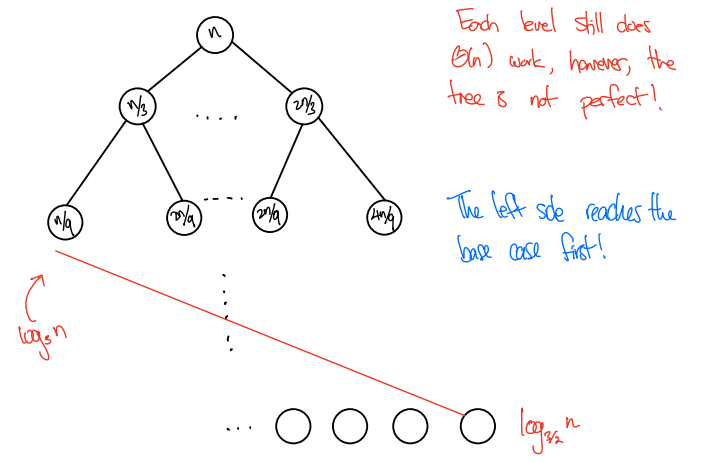
\includegraphics[scale=0.5]{recursion-tree1.png}
\end{center}
Our \textbf{lower bound} is when we remove all nodes with height $> \log_3(n)$. Then, the remaining tree is perfect, has height $\log_3(n)$, and $n$ work at each level. So, we guess $\Theta(n \log(n))$.\\
Our \textbf{upper bound} is when levels below $\log_3(n)$ also do $n$ work. Then, we do $n$ work for $\log_{3/2}(n)$ levels. So, we guess $\Theta(n \log(n))$.\\
We can then prove both of these bounds using substitution.

\subsection{Standard Form Recurrences}
A recurrence is in \textbf{standard form} if it is written as:
$$T(n) = aT(n/b) + f(n)$$
For some constants $a \geq 1, b > 1$, and some function $f: \mathbb{N} \to \mathbb{R}$\\
Most divide-and-conquer algorithms will have recurrences that look like this.

\subsubsection{Standard Form Parameters}
$$T(n) = aT(n/b) + f(n)$$
\begin{enumerate}
    \item $a$: The \textbf{branching factor} of the tree: How many children does each node have?
    
    \item $b$: The \textbf{reduction factor}: How much smaller is the sub-problem in the next level of the tree compared to this level?
    
    \item $f(n)$: The \textbf{non-recursive work}: How much work is done outside of the recursive call on inputs size $n$? We make the assumption that $f$ is positive and non-decreasing.
\end{enumerate}

\subsubsection{Standard Form and Recursion Trees}
Recursion trees can also be used for standard form recurrences.
\begin{enumerate}
    \item What is the height of the tree? | $\log_b(n)$
    \item What is the number of vertices at height $h$? | $a^h$
    \item Total non-recursive work at level $h$? | $f(n)$ (the root), and $a^{\log_b(n)} \cdot f(1) = \Theta(n^{\log_b(a)}$ (the leaf)\\
    In total, it is $a^h f(n/b^h)$
\end{enumerate}
Altogether, the total amount of work done is $\sum_{h = 0}^{\log_b(n)} a^h f(n/b)$.

\begin{center}
    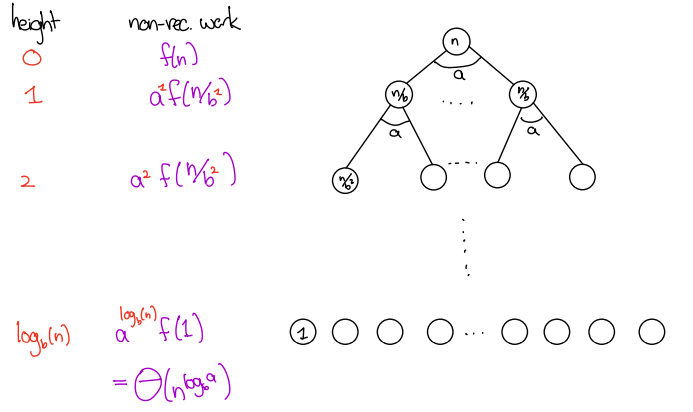
\includegraphics[scale=0.6]{imgs/standard-form-tree.png}
\end{center}

\subsection{Master Theorem}
Thm. Let $T(n) = aT(n/b) + f(n)$. Define the following cases based on how the root work compares with the leaf work.
\begin{enumerate}
    \item \textbf{Leaf heavy:} $f(n) = O(n^{\log_b(a) - \epsilon})$ for some constant $\epsilon > 0$.
    \item \textbf{Balanced:} $f(n) = \Theta(n^{\log_b(a)})$
    \item \textbf{Root heavy:} $f(n) = \Omega(n^{\log_b(a) + \epsilon})$ for some $\epsilon > 0$, and $a f(n/b) \leq cf(n)$ for some constant $c < 1$ for all sufficiently large $n$. 
\end{enumerate}
Then, we have:
$$T(n) = \begin{cases}
\Theta(n^{\log_b(a)}) & \text{Leaf heavy case}\\
\Theta(n^{\log_b(a)} log(n)) & \text{Balanced case}\\
\Theta(f(n)) & \text{Root heavy case}
\end{cases}$$
$f(n) = O(n^{\log_b(a) - \epsilon})$ for some $\epsilon > 0$ means that $f(n)$ is smaller than $n^{\log_b(a)}$ by a factor of at least $n^\epsilon$.\\\\
For example, if $log_b(a) = 2$, then $n^{1.9} = O(n^{2 - \epsilon})$ for some $\epsilon >0$, but $n^2/\log(n) \neq O(n^{2-\epsilon})$ for any $\epsilon > 0$, even though $n^2/\log(n) = o(n^2)$.

\subsubsection{Additional Regularity Condition}
The condition in the root for the \textbf{heavy case} that $af(n/b) \leq cf(n)$ for some constant $c < 1$ for all sufficiently large $n$ is called the \texbtf{regularity condition}.\\
\\
In the root heavy case, most of the work is done at the root. $af(n/b)$ is the total work done at level $1$ of the tree. The regularity condition says if most of the work is done at the root, we do more at the root than at level 1 of the tree.

\subsubsection{Proof of Master Theorem}
Geometric Series is the sum:
$$S = a + ar + ar^2 + ... ar^{n-1} = \sum_{i=0}^{n-1}ar^i$$
i.e., each term in the sum is obtained by multiplying the previous term by $r$. The closed-form solution for $S$ is
$$S = a\left( \frac{r^n - 1}{r-1}\right)$$
To prove this, just rearrange: $rS = ar + ar^2 + ar^n = S + ar^n - a$.\\
\\
So, to prove the Master Theorem, we analyze the recursion tree for the generic standard form recurrence. That is, $f(n) = \Theta(n^{\log_b(a)}$.\\
We have multiple cases:
\begin{enumerate}
    \item Balanced Case\\
    Suppose we have a tree, and the heights go as follows:
    \begin{center}
        \begin{tabular}{c|c}
            Height & Non-Recursive Work \\
            \hline
            0 & $f(n)$\\
            1 & a^1 \ $f(n/b^1) \ = \ a/a \cdot n^{\log_b a} \ = \ n^{\log_b(a)}$\\
            2 & a^2 \ $f(n/b^2) \ = \ a^2/a^2 \cdot n^{\log_b a} \ = \ n^{\log_b(a)}$ \\
            ... & ...\\
            $\log_b(n)$ & $a^{\log_b(n)}f(1) \ = \ n^{\log_b(a)}$
        \end{tabular}
    \end{center}
    Where $a^{\log_b(n)}f(1) = \Theta(n^{\log_b a)}$.\\
    So, in total we have:
    $$\log_b(n) \cdot n^{\log_b a} = \Theta(n^{\log_b a} \cdot \log(n))$$
    \item Leaf-Heavy Case
    \begin{center}
        \begin{tabular}{c|c}
             Height & Non-Recursive Work \\
             \hline
             0 & n^{\log_b(a)}/n^\epsilon\\
             1 & a(n/b)^{\log_b(a)} / (n/b)^\epsilon\\
             2 & a^2(n/b^2)^{\log_b(a)} / (n/b^2)^\epsilon\\
             ... & ... \\
             \log_b(n) & \Theta(n^{\log_b(a)}
        \end{tabular}
        Using the geometric series with the ration $b^\epsilon$ and $\log_b(n)$ terms, we have in total:
        \begin{align*}
            (n^{\log_b(a)}/n^\epsilon)(1 + b^2 + b^{2\epsilon} + ... + b^{(\log_b(n) - 1)\epsilon}) + \Theta(n^{\log_b(a)}\\
            & = (n^{\log_b(a)}/n^\epsilon) \cdot (\frac{(b^\epsilon)^{\log_b(n)} - 1}{b^\epsilon - 1}) + \Theta(n^{\log_b(a)}\\
            & = (n^{\log_b(a)}/n^\epsilon) \cdot \Theta(n^\epsilon) + \Theta(n^{\log_b(a)}\\
            & = \Theta(n^{\log_b(a)}
            \end{align*}
    \end{center}
    \item Root-Heavy Case: Similar to previous cases.
\end{enumerate}

\subsubsection{Applying the Master Theorem}
\begin{enumerate}
    \item Write the recurrence in standard form to find the parameters $a,b,f$.
    \item Compare $n^{\log_b(a)}$ to $f$ to determine the case split.
    \item Read off the asymptotics from the relevant case.
\end{enumerate}

\subsection{Summary of Recurrence Methods}
\begin{center}
    \setlength{\tabcolsep}{0.6em} % for the horizontal padding
    {\renewcommand{\arraystretch}{1.4}% for the vertical padding
    \begin{tabular}{| p{3cm} | p{4cm} | p{8cm} |}
         \hline
         \textbf{Method} & \textbf{Pros} & \textbf{Cons} \\
         \hline
        Induction & Always works, can get more precision & Requires a guess, can get technical. Complex proofs.\\ 
        \hline
        Substitution & Always works & Requires a guess and is slower than others.\\
        \hline
        Recursion Trees & Intuitive & Doesn't always work, but a good starting point and good for generating guesses.\\
        \hline
        Master Theorem & Proofs are very short & Restricted scope (recurrences must be in standard form and fall into one of the cases).\\
        \hline
    \end{tabular}
    }
\end{center}

\section{Correctness}
We can prove algorithms that are "correct" in the sense that they do what we expect them to do. We use CS/Python notation.
\begin{enumerate}
    \item Elements of a list of length $n$ are $l[0], l[1], ..., l[n-1]$
    \item Slicing: $l[i:j] = [l[i], l[i + 1], ..., l[j - 1]]$\\
    By convention, if $j \leq i$, then $l[i:j] = []$.
\end{enumerate}

\subsection{Merge Sort Correctness}
We can show $merge\_sort$ works on every input using induction.\\
Break down the function and show for all $n \in \mathbb{N}, merge\_sort$ works on inputs of size $n$.\\
\\
Let $P(n)$ be the predicate: Let $l \in [\mathbb{N}]$ be a list of natural numbers of length $n$, then $merge\_sort(l)$ returns the sorted list.\\
Claim. $\forall n \in \mathbb{N}, P(n)$
\begin{proof}
For now, assume $merge$ is correct. \\
Base Case. Let $l$ be a list length $0$ or $1$. In this case, $\merge\_\sort(l)$ returns $l$ as expected.\\
\\
Inductive Step. Let $k \in \mathbb{N}$ with $k \geq 1$, and assume for all $i \in \mathbb{N}$ with $0 \leq i \leq k$, $\merge\_\sort$ works on lists of length $i$. We WTS $\merge\_\sort$ works on lists length $k + 1$. Let $l$ be a list of length $k + 1$.\\
Since $k + 1 \geq 2$, we fall into the else case of the function. The left sublist is a list length $\lfloor(k+1)/2\rfloor$. We have:
\begin{align*}
    \lfloor(k+1)/2\rfoor & \leq (k+1)/2 \\
    & \leq (k + k)/2 & (k \geq 1)\\
    & \leq k
\end{align*}
Then, by inductive hypothesis, $\merge\_\sort$ correctly sorts the left sublist, and $\Left$ contains the sorted left sublist.\\\\
Then, the right sublist is a list of length $k + 1 - \lfloor(k+1)/2\rfloor$. Since $k \geq 1, \lfloor(k+1)/2\rfloor \geq 1$.\\
Thus, $k + 1 - \lfloor(k+1)/2\rfloor \leq k + 1 - 1 = k$.\\
Hence, by inductive hypothesis, $\merge\_\sort$ correctly sorts the right sublist, and $\Right$ contians the sorted right sublist.\\
Since we're assuming $\merge$ works, and $\Left$, $\Right$ are sorted lists, with $l$ being composed of elements in $\Left$, $\Right$, we can return $\merge(\Left, \Right)$ which is the sorted version of $l$.
\end{proof}

\subsection{Binary Search Correctness}
Let $P(n)$ be the predicate: For all lists $l \in List[\mathbb{N}]$ and $t \in \mathbb{N}$, if $b - a = n$, then $bin\_search(l,t,a,b)$ returns $None$ is $t$ is not in $l[a:b]$, and the index of $t$ in $l$ otherwise.\\
Claim. $\forall n \in \mathbb{N}, P(n)$.
\begin{proof}
Base Case. Consider $n = 0$. Let $l$ be any list and suppose $b-a = 0$. Then $l[a:b] = []$, so $t$ is not in $l$, and we expect the algorithm to return $None$.\\
Indeed, since $b == a$, the first $if$ check passes, and $bin\_search(l,t,a,b)$ returns $None$.
\\
Inductive Step. Let $k \in \mathbb{N}$ and assume for all $i \in \mathbb{N}, i \leq k, P(i)$. We WTS $P(k+1)$, and let $l \in \List[\mathbb{N}]$ be a sorted list, and $t,a,b \in \mathbb{N}$ such that $b - a = k+1$.\\
We show that $bin\_search(l,t,a,b)$ returns $None$ if $t$ is not in $l[a:b]$ and the index of $t$ in $l$ otherwise.\\
Since $b - a = k + 1 \geq 1$, the first $if$ check fails. Let $m = (a+b) //2 = \lfloor(a+b)/2\rfloor$. Then, there are 3 cases:
\begin{enumerate}
    \item \begin{verbatim}
        l[m] == t
    \end{verbatim}
    In this case, the algorithm returns $m$, which is the index of $t$ in $l$.\\
    We need to check $l[m] = t$ is actually in $l[a:b]$, i.e., that $a \leq m \leq b -1$.
    \begin{align*}
        m & = \lfloor(a+b)/2\rfloor\\
        & \geq \lfloor(2a+1)/2\rfloor & (b-a \geq 1)\\
        & \geq \lfloor a + (1/2)\rfloor\\
        & \geq a
    \end{align*}
    On the other side:
    \begin{align*}
        m & = \lfloor (a+b)/2 \rfloor\\
        & \leq \lfloor (2b-1)/2 \rfloor & (b-a \geq 1)\\
        & \leq \floor b - (1/2)\rfloor\\
        & = b-1
    \end{align*}
    
    \item \begin{verbatim}
        l[m] < t
    \end{verbatim}
    Since $l$ is sorted and $t$ is greater than $l[m]$, if $t$ is to be in $l[a:b]$, it must have an index greater than $m$. So: $bin\_search(l,t,a,b) = bin\_search(l,t,m+1, b$.\\
    We claim that the IH applies to $bin\_search(l,t,m+1,b)$. We just need to show $b - (m+1) \leq k$.\\
    We know from the previous part that $m \geq a$, so then:
    $$b - (m+1) \leq b - (a+1) \leq b - a - 1 = k$$
    
    \item \begin{verbatim}
        l[m] > t
    \end{verbatim}
    Since $l$ is sorted and $t$ is less than $l[m]$, if $t$ is to be in $l[a:b]$, it has an index less than $m$. So: $bin\_search(l,t,a,b) = bin\_search(l,t,a,m)$.\\
    We claim our IH applies to $bin\_search(l,t,a,m)$. We WTS $m-a \leq k$.\\
    From the previous part, we know $m \leq b - 1$. Then:
    $$m - a \leq b - 1 - a \leq k$$
    so the inductive hypothesis holds for $bin\_search(l,t,a,m)$.
\end{enumerate}
\end{proof}

\subsection{Proving Correctness}
For any algorithm/function/program, define a precondition and postcondition.
\begin{enumerate}
    \item The precondition is an assertion about the inputs to a program.
    \item The postcondition is an assertion about the end of a program.
\end{enumerate}
An algorithm is correct if the precondition implies the postcondition (i.e., for valid inputs, your algorithm should give me the expected outputs.

\subsubsection{Examples of Correctness}
\begin{enumerate}
    \item $merge\_sort(l)$:\\
    Precondition: $l$ should be a list of natural numbers.\\
    Postcondition: The return value of $merge\_sort(l)$ in sorted order.
    
    \item $bin\_search(l,t,a,b)$\\
    Precondition: $l \in \List[\mathbb{N}]$, $l$ is sorted, $t,a,b \in \mathbb{N}$, $a,b \leq \len(l)$.\\
    Postcondition: If $t$ is in $l[a:b]$, return the index of $t$ in $l$, otherwise, return $\None$.
\end{enumerate}

\subsection{Iterative Algorithms}
Iterative algorithms are algorithms with while or for loops.\\
Conventions:
    \begin{enumerate}
        \item Iteration numbers start at 0.
        \item Beginning of iteration $n$ is the same as `end of iteration $n-1$'.
        \item Thus, a for loop with iteration $0, ..., n-1$ reaches the start of the $n'$th iteration.
    \end{enumerate}\\

To show correctness, the general strategy is to define a loop invariant - some property that is true at the start of every iteration - note that it can depend on the iteration number. Call it $P(n)$.\\
Since the value of variables in code can change at each iteration, it is useful to refer to the value of a variable at certain iterations using the iteration number as a subscript.\\
Prove the loop invariant holds by induction and show the loop invariant holds at the end of the loop (implying the post condition).\\
Sometimes, instead of base case and inductive step, the following terminology is used:
\begin{enumerate}
    \item \textbf{Initialization.} Show the loop is true at the start of the loop (base case).
    \item \textbf{Maintenance.} Show that if the loop invariant is true at the start of any iteration, it is true at the start of the the next iteration (inductive step).
    \item \textbf{Termination.} Show that the loop terminates (important for while loops), and that when the loop terminates, the loop invariant implies what we want (the postcondition).
\end{enumerate}
\subsubsection{Example of Iterative Correctness}
Take $mult(x,y)$, a function that adds $x$ to the total $y$ times.\\
Precondition:  $x,y \in \mathbb{N}$\\
Postcondition: Return $x \cdot y$.\\
\\
To prove this is correct, we show that the precondition implies the postcondition. Namely, that if $x,y \in \mathbb{N}, mult(x,y)$ returns $xy$.
\begin{proof}
    Let $total_n$ be the value of the variables total at the start of the $n$th iteration.\\
    Let $P(n)$ be $total_n = xn$. We WTS $\forall n \in \mathbb{N}, P(n)$.\\
    \\
    Base Case. Consider the value of $total$ before the start of the for loop. Note the total is initialized to 0, which is equal to $x \cdot 0$, as required.\\
    \\
    Inductive Step. Let $k \in \mathbb{N}$ with $k \leq y-1$. Assume $total_k = xk$. Now consider the execution of iteration $k$.\\
    The contents of the for loop increment the value of $total$ by $x$. Thus, $total_{k+1}$, the value of total at the start of iteration $k+1$ is:
    \begin{align*}
        total_{k+1} & = total_k + x\\
        & = xk + x & (IH)\\
        & = x(k+1)
    \end{align*}\\
    The last iteration of the for loop is $n = y-1$, therefore, at the end of this iteration (the start of iteration $y),$ the value of $total$ is $x \cdot y$. We then return the value of total, so $mult(x,y)$ returns $xy$ as required.
\end{proof}
For the runtime, suppose $x,y$ are $n$-digit numbers, and it takes $O(n)$ time to add two $n$ digit numbers. The worst-case time complexity would be $10^n - 1 \in \Theta(10^n)$, since $y$ is an $n-$digit number as large as $9999...99$ (n-times).\\
The eventual result has at most $2n$ digits. Thus, each addition takes $O(2n) = O(n)$. In total, the runtime is $\Theta(n10^n)$.

\subsubsection{While Loops}
While loops are typically more difficult to prove the correctness of. Specifically, you need to prove the while loop terminates.\\
There are two ways to check correctness:
\begin{enumerate}
    \item Create a property for the loop invariant that implies the while check will fail at iteration $n$ for some $n \in \mathbb{N}$.
    \item Use the fact that any strictly decreasing sequence of natural numbers is finite to define some variable $x \in \mathbb{N}$, and argue that it decreases with every iteration of the while loop.\\
    The execution of the while loops defines a decreasing sequence of natural numbers so that it terminates.
\end{enumerate}
\\
\underline{Example of Strictly Decreasing Sequence of Natural Numbers:} Take the mystery function. For $x,y \in \mathbb{N}, y>0$ the algorithm returns $\lceil x/y\rceil$. \\
To prove its descending sequence, assume the claim is true at the start of iteration $k$ and show it is true at the start of iteration $k+1$. We have:
\begin{align*}
    a_{k+1} & = x+y - val_{k+1}\\
    & = x+y - val_k - y\\
    & = a_k - y\\
    & < a_k & (y>0)
\end{align*}
Furthermore, cancelling the $y$'s in the second line, we get $a_{k+1} = x - val_k$, which is greater thatn $0$ since the while check passes. This combined with the fact that $y \in \mathbb{N}$ and $a_k \in \mathbb{N}$ implies that $a_{k+1} \in \mathbb{N}$.\\
Thus, $a_n$ is indeed a decreasing sequence of natural numbers.\\
\\
Now, we determine the loop invariant.\\
Let $val_n, c_n$ be the real value of $val$ and $c$ at the start of iteration $n$. By convention, the iteration number starts at $0$.\\
Let $P(n)$ be the predicate that is true if and only if $val_n = c_ny$ at the start of the iteration $n$, and $c_n = n$.
\begin{proof}
Initializtion. At the start of iteration 0, $val_0 = c_0 = 0$, as required.\\
\\
Maintenance. Assume the loop invariant holds at the start of some iteration $k$, and show it holds at the start of iteration $k$, and show it also holds at the start of iteration $k+1$. By the end of the iteration $k$, $val$ was incremented by $y$ and $c$ is incremented by $1$, so:
$$val_{k+1} = val_k + y, \ \ \ c_{k+1} = c_k+1$$
Applying the loop invariant to iteration $k$, we have:
$$val_{k+1} = c_k \cdot y + y = (c_k + 1)y = c_{k+1}y$$
as required.\\
\\
Termination. Since the algorithm terminates, let $k$ be the iteration number such that the check in the while loop fails. We return $c_k = k$. Thus it suffices to show $k = \lceil x/y \rceil$.\\
Since the check fails for iteration $k$ and passes for iteration $k-1$, we have
$$ky \geq x, \ \ \ (k-1)y < x$$
Putting the two together, we have:
$$\frac{x}{y} \leq k < \frac{x}{y} + 1$$
i.e., $k$ is the natural number that is at least $\frac{x}{y}$ and less than $\frac{x}{y} + 1$, so $k = \lceil x/y \rceil$, as required.
\end{proof}
\\
\underline{Using the Loop Invariant}
Suppose the algorithm does not terminate. Then, it at least reaches iteration $x$.\\
$P(x) \implies val_x = xy \geq x$, so the while loop check fails and the algorithm terminates, which is a contradiction. \\
\\
Take the algorithm $merge$, where $x,y$ are sorted lists, and the algorithm returns a sorted lists with elements from $x$ and $y$.\\
In this case, the descending sequence is $len(x) + len(y) - len(l)$, and the loop invariant is that $l,x,y$ are all sorted and for all $a \in l, b \in x + y, a\leq b$, i.e., all the elements are not yet added to $l$, come after all the elements added to $l$.\\
To show termination, define a sequence of natural numbers that decrease with every iteration. So, let $x_i, y_i, l_i$ be the values of $x,y,l$ at the start of iteration $i$. Again, use the convention that the iteration starts at $0$.\\
We claim that
$$a_n = len(x_0) + len(y_0) - len(l_n)$$
has this property. To show this, it suffices to show that $len(l)$ is increasing with each iteration and is at most $len(x) + len(y)$.\\
If either of the two if conditions pass, we return, and so the loop finishes. In the other two cases,a  new element gets appended to $l_n$, and hence $len(l_{n+1}) > len(l_n)$.\\
Note that since all elements can get appended to $l$ come from either $x$ or $y$, $len(l_n) \leq len(x) + len(y)$.\\
\\
For our loop invariant, we have $P(n)$:
\begin{enumerate}
    \item $l_n, x_n, y_n$ are sorted.
    \item $\forall b \in x_0 + y_0, b$ is in exactly one of $x_n, y_n, l_n$
    \item $\forall a \in l_n, \forall b \in x_n + y_n, a \leq b$.
\end{enumerate}
\begin{proof}
Initialization.
\begin{enumerate}
    \item $l_0$ is empty so it is vacuously sorted. $x_0$ and $y_0$ are sorted by that precondition.
    \item let $b \in x_0 + y_0$. If $b$ was in $x_0$, then it is in $x_0$, and if $b$ was in $y_0$, it is in $y_0$.
    \item $l_0$ is empty so 3 holds vacuously.
\end{enumerate}
Maintenance: Assume $P$ holds at the start of iteration $k$, we WTS it also holds at the end of iteration $k$.\\
In this section, we only consider branches that don't end the loop. If $x_k[0] \leq y_k[0]$, we have:
\begin{enumerate*}
    \item $x_{k+1} = x_k[1:]$
    \item $y_{k+1} = y_k$
    \item $l_{k+1} = l_k + [x_k[0]]$
\end{enumerate*}
So:
\begin{enumerate}
    \item Holds at the end of the iteration, since 3 holds at the start of iteration $k$.
    \item Holds since 2 holds at the start of the iteration, and we simply moved one element from $x$ to $l$.
    \item Holds at the end of iteration $k$ since 1 and 3 hold at the start of iteration $k$; $x_k[0]$ is minimal in $x_k + y_k$.
\end{enumerate}
The else case for this is similar.\\
\\
Termination. We already have shown the algorithm terminates. Suppose $k$ is the iteration in which the loop terminates. The only way the while loop exists is if we reach one of the first two cases.\\
If the first case is reached, $len(x_k) = 0$ and we return $l_k + y_k$. Since the loop invariant holds at the start of the iteration, every element originally in $x_0$ or $y_0$ is in either $l_k$ and $y_k$.\\
By (3) of the loop invariant, every element in $y_k$ is at least every element of $l_k$. Furthermore, since $l_k + y_k$ are sorted by (1) of the loop invariant, $l_k + y_k$ is indeed a sorted list containing every element in $x_0 + y_0$.\\
The second case is similar, and thus the postcondition is satisfied when the algorithm terminates.
\end{proof}

\section{Finite Automota and Modeling Computations}
We previously showed using Cantor's Theorem that there are problems that cannot be solved, defining a problem for each set.\\
If $A$ is a set of strings, there is the problem of deciding whether a given input is in $A$ or not. For example:
$$A = \{w \in \Strings: w \text{ is a palindrome} \},$$
$$A = \{w: w \text{ is a C program with no syntax errors.}\}$$

\subsection{Language Definitions}
We solve problems with languages utilizing the following definitions:
\begin{enumerate}
    \item An \textbf{alphabet}, $\sum$, is a non-empty, finite set of symbols.\\
    For example: $\{0,1\}$, $\{a,b,c,d,...,z\}$.
    \item A \textbf{string} $w$ over an alphabet $\sum$ is a finite (0 or more) sequence of symbols from $\sum$.
    \item The set of all strings is denoted as $\sum^*$.
    \item A \textbf{language} is any subset of $\sum^*$, denoted as $L \subseteq E^*$.
    \item We denote the empty string by $\epsilon$.
\end{enumerate}

Given a language $A$ over the alphabet $\sum$, come up with a program that determines whether or not an input string $x \in \sum^*$ is in $A$ or not.

\subsection{Determinite Finite Automota}
Determining a function that finds this answer can be very difficult and complicated, so we want to try to find a better way of determining different programs in its simplest and most ``bare-bones'' way.
    \begin{center}
        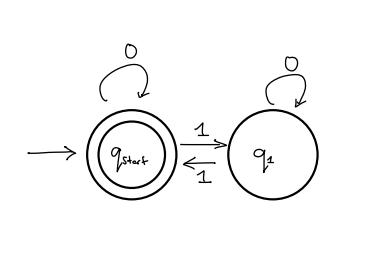
\includegraphics[scale=0.6]{imgs/finite-automota.png}
    \end{center}
    Input: A string $w \in \sum^*$.\\
    Output: An accept/reject.
    \begin{enumerate}
        \item The DFA starts at a predefined starting state.
        \item The DFA reads the input tring one character at a time. Depending on the character read and the current sate, the DFA \textit{deterministically} moves to a new state.
        \item Once it reads the entire string, the DFA will be in some state. If that state is one of the accept states, the DFA accepts. Otherwise, the DFA rejects.
    \end{enumerate}
    \begin{center}
        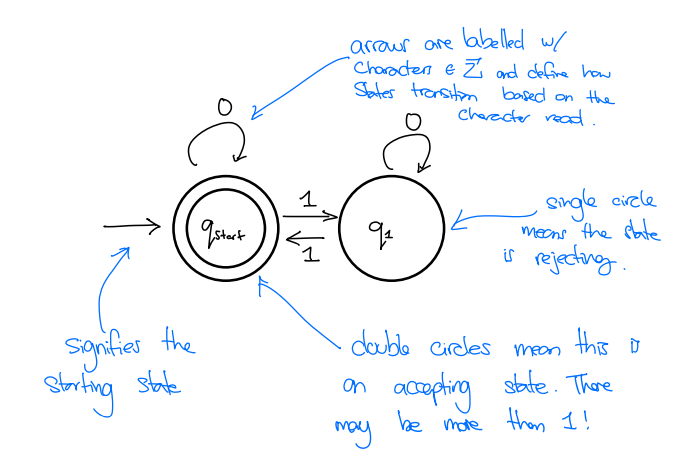
\includegraphics[scale=0.6]{imgs/finite-automota-labeled.png}
    \end{center}
    Let $M$ be a DFA, the \textbf{language of DFA}, denoted as $L(M)$ is the set of strings $w \in \sum^*$ such that $M$ accepts $w$.\\
    Then, We take a language $A \subseteq \sum^*$, and find a DFA $M$ such that $L(M) = A$.\\
    \\
    DFAs are deterministic, meaning that for the given state and character read, the next state is always the same. They are also finite. which means they have a finite number of states. States are analogous to memory, since we can store information about the input by transitioning to different states.
    
    \subsubsection{Examples of DFAs}
    \begin{enumerate}
        \item \begin{center}
            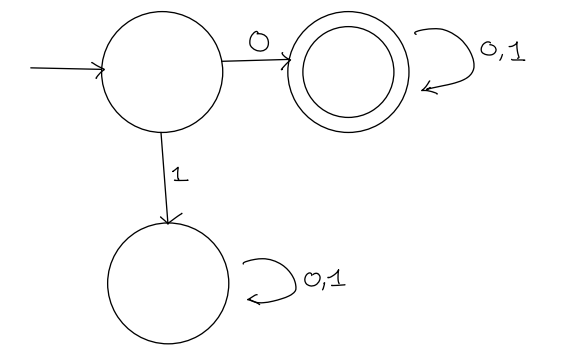
\includegraphics[scale=0.5]{imgs/dfa-example1.png}
        \end{center}
        This accepts any string that starts with `0'.
        
        \item \begin{center}
            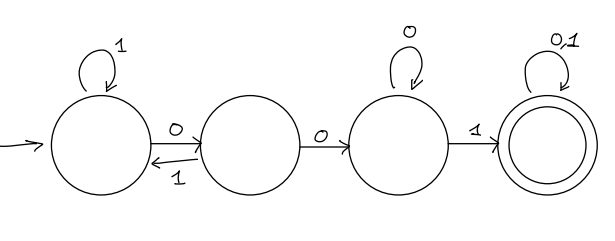
\includegraphics[scale=0.5]{imgs/dfa-example2.png}
        \end{center}
        This accepts any string that contains `001'. That is: $L(M) = \{w: 001 \in w\}$.
        
        \item \begin{center}
            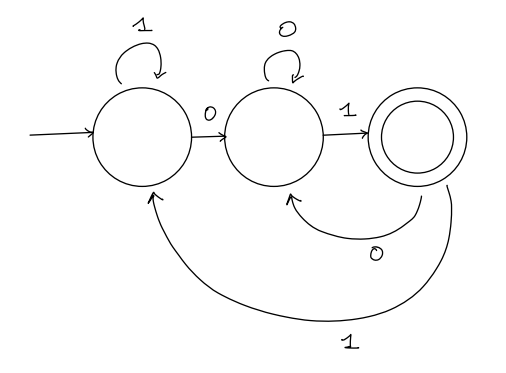
\includegraphics[scale=0.5]{imgs/dfa-example3.png}
        \end{center}
        This accepts any string that ends with `01'.
    \end{enumerate}
    \subsubsection{Designing DFAs}
    \begin{enumerate}
        \item State the alphabet $\sum$ of the DFA.
        \item Define a finite set of states, $Q$.
        \item State the start state $q_{start} \in Q$.
        \item Write which states are accepting, and formally find a subset $F \subseteq Q$ of accept states.
        \item For each state $q$ and each character $x \in \sum$, state which class to go to next if you read $x$ from state $q$.
    \end{enumerate}
    
    \subsection{Nondeterminate Finite Automota}
    NFAs are similar to DFAs, with a few key differences.
    \begin{center}
        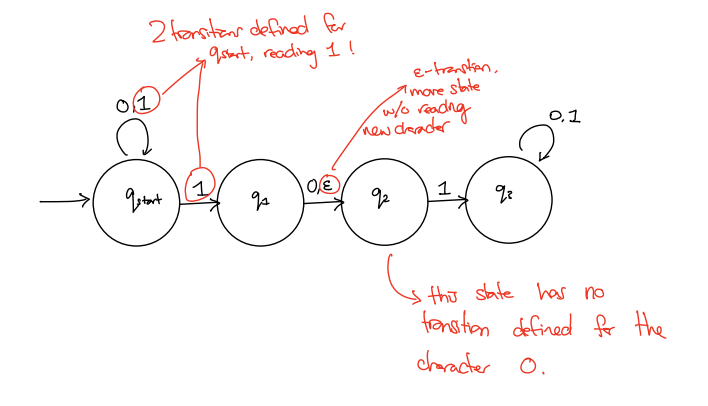
\includegraphics[scale=0.6]{imgs/nfa-labeled.png}
    \end{center}
    Input: A string $w \in \sum^*$.\\
    Output: An accept/reject.
    \begin{enumerate}
        \item The NFA starts at a predefined start state.
        \item The NFA reads in the input string one character at a time.\\
        Let $c$ be the character that was read. There are several cases depending on the current state:
        \begin{enumerate}
            \item If the state has no arrows coming out of it labelled with $c$, immediately reject.
            \item Otherwise, choose one of the arrows labelled with $c$ and follow it.
        \end{enumerate}
        \item When it has read the entire string, the NFA will be in a particular state. Depending on the choices made, the final state will either be accepting or rejecting.\\
        The NFA accepts the string if any sequence of choices leads to an accept state.
    \end{enumerate}
    
    \subsubsection{Differences Between DFAs and NFAs}
    \begin{enumerate}
        \item For each state, there can be multiple arrows labelled with the same character.
        \item Arrows can be labelled with $\epsilon$ (empty string).
        \item States do not need to have one arrow for each character in $\sum$.
    \end{enumerate}
    
    \subsection{Regular Languages}
    A language $A$ is \texbtf{regular} if and only if there is a DFA $M$ such that $L(M) = A$.
    
    \subsubsection{Language Operations}
    We have for languages $A,B$ over $\sum^*$:
    \begin{enumerate}
    \item The \textbf{complement} of $A$, denoted $\overline{A} = \sum^* \setminus A$
    
    \item The \textbf{concatenation} of $A, B$ denoted $AB = \{ab: a \in A, b \in B\}$, which is the set of strings you get by concatenating a string in $A$ and a string in $B$.
    
    \item $A^n = \{a_0a_1, ..., a_{n-1} : a_0 \in A, a_1 \in A, ..., a_{n-1} \in A\}$.\\
    In other words, it is $A$ concatenated with itself $n$ times; i.e., it is the set of strings you get by concatenating $n$ strings in $A$.\\
    Note $A^0 = \{\epsilon\}$ for all $A$, and $A^1 = A$.
    
    \item $A^* = \cup_{i\in\mathbb{N}}A^i$: The \textbf{Kleene star} of $A$. We typically say $A$ star.\\
    Note that $\epsilon \in A^* \forall A \subseteq \sum^*$.
    
    \item $A \cup B$, $A \cap B$ are the union and intersection.
    \end{enumerate}
    
    \subsubsection{Finite Languages}
    Let $w \in \sum^*$ be any string. Then, $\{w\}$ is a regular.
    \begin{proof}
    Since $\sum^*$ is finite, we have $w = w_1, w_2, ..., w_n$.\\
    We construct our DFA where transitions that are not $w$ reach a dead end, and everything else is the accept state.
    Then $\{w\}$ would be the regular.
    \begin{center}
        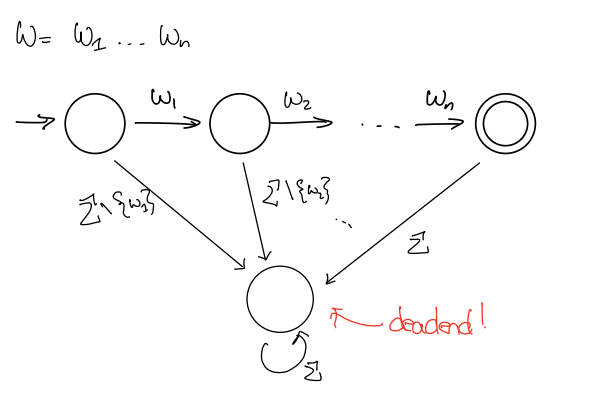
\includegraphics[scale=0.5]{imgs/finite-language-regular.png}
    \end{center}
    \end{proof}
    
    \subsubsection{NFAs and Regular Languages}
    We re-iterate that nondeterminism is if any sequence of choices leads to an accept state, accept. Reject only if every sequence of choices leads to reject. Then, we can choose which transitions to take.\\
    \\
    Theorem. Let $A$ be any language. There is a DFA $M$ such that $A = L(M) \iff \exists$ NFA $N$ such that $A = L(N)$.
    \begin{proof}
        \begin{enumerate}
            \item $\implies$: We know that every DFA is an NFA, so we know this is true. 
            
            \item $\impliedby$: We simulate a NFA $N$ with DFA $M$.\\
            We have a state in $M$ for every subset of states in $N$. Let $S, T$ be two states in $M$. Then $S$ transitions to $T$ reading $\sigma$ if some choice allows me to go from a state in $S$ to a state in $T$. This choice includes an unlimited amount of $\epsilon$ transitions.\\
            Then, the accept states are the subsets that contain accept states, and the start state is the subset containing the start state in $N$ and all states reachable from the start state using an $\epsilon$ transition.\\
            More intuitively, if you are at state $S$ after reading $w$, $S$ should contain all states you could have been in $N$.
        \end{enumerate}
    \end{proof}
    
    The more complex a model of computation is, the easier it is to use. Then, NFAs are more complex so finding the NFAs for a language is easier than finding DFAs for a language.\\
    However, the more limited the model of computation is, the easier it is to prove things about. DFAs are very restrictive, so a lot of properties can be proved.\\
    However, since these two models of computation are equivalent, we can pick the right model for different situations.\\
    \\
    For instance:
    \begin{center}
        $A$ is regular $\iff$ $\exists$ DFA $M$ such that $L(M) = A$ $\iff$ $\exists$ NFA $N$ such that $L(N) = A$
    \end{center}
    
    
    \subsubsection{Closure}
    Suppose $A, B$ regular languages. Then:
    \begin{enumerate}
        \item $\overline{A}$
        \item $AB$
        \item $A \cup B$
        \item $A \cap B$
        \item $A^n$, and
        \item $A^*$
    \end{enumerate}
    are all regular.
    \begin{proof}
    We also know for a fact that finite languages themselves are regular.
    \begin{enumerate}
        \item $\oveline{A}$: Suppose $A$ is regular. Then, let $M$ be a DFA for $A$.\\
        Let $M'$ be the DFA with all the states of $M$ flipped. Then $L(M') = \overline{A}$.\\
        Informally, we know that if $w \in L(M)$, this means that it's reached the final accept state, implying that $w \not\in L(M')$ since all accepts turn into rejects, and vice-versa.
        
        \item $A \cup B$: Let $M, N$ be DFAs for $A,B$ respectively. We want to find a DFA $D$ for $A \cup B$.\\
        Here, we can run our DFAs in parallel, making each state in our DFA $D$ correspond to a 2-tuple $(M, N)$.\\
        Then, at state $(x,y)$, we read character $\sigma$, and then transition to $(x', y')$, where $x'$ is the state $x$ goes into in $M$ when reading $\sigma$, and $y'$ is the state that $y$ goes into in $N$ when reading $\sigma$.\\
        Then, the accepting state occurs if either $x$ was an accept state in $M$ or $y$ was an accept state in $N$ (or both).\\
        \\
        When we construct these states for the union, sometimes we get ``extra'' states that are never used but the language is still valid.
         
         \item $A \cap B$: Something that is proven in homework.
         
         \item $AB = \{ab: a \in A, b \in B\}$: The same trick of running DFAs in parallel can't work, so writing this as a function, for each input, we try to split up the string in different ways such that the first half is in $A$, and the second half is in $B$, then accept. If there is no way to split up the string, reject.\\
         We can guess where the string in $A$ ends and when the string in $B$ starts using NFAs.\\
         Let $M,N$ be DFAs for $A,B$ r4respectively. We show that $AB$ is regular by finding an NFA $H$ for $AB$.\\
         So, we take the accept states for the first half of the input for $M$ and use $\epsilon$ transitions to go into the second half of the input for $N$.\\
         Then, if $w \in L(H)$, then $w \in AB$.
    \end{enumerate}
    \end{proof}
    
    \subsection{Non-Regular Languages}
    We know that DFAs have a finite number of states, and we know that states correspond to memory. Then, intuitively, DFAs can compute languages that need a finite amount of memmory.\\
    In particular, a DFA has a \texbtf{fixed amount of memory} no matter how large the input is.\\
    \\
    For example, \textbf{Even} is regular because no matter how large the input is, you just need to store one bit corresponding to whether it has an even number of 1s or not.\\
    \\
    However, languages such as
    $$X = \{a^nb^n : n \in \mathbb{N}\}$$ 
    can NOT be solved using finite memory, since you continuously need more memory.\\
    To prove this is not regular, we need to prove there does not exists a DFA $M$ such that $L(M) = X$, but this is near-impossible. So, we can use a theorem to prove this.
    
    \subsubsection{Myhill-Nerode Theorem}
    \paragraph{Indistinguishable Key - }\\
    Let $A$ be a language over $\sum$. For any strings $x,y,w \in \sum^*$, call $w$ a \textbf{distinguisher} for $x,y$ if exactly one of $xw$ and $yw$ is in $A$.\\
    That is, a DFA for $A$ accepts one of $xw$ and $yw$, and rejects the other.\\
    \\
    We can define the binary relation $\sim_A$ over $\sum^*$ where for any $x,y \in \sum^*$:
    $$x \sim_A y \iff \neg\exists \text{a distinguisher for x and y}$$
    In English, we say $x$ is \textbf{indistinguishable} from $y$ relative to $A$.\\
    \\
    We know that $\sim_A$ is an equivalence relation over $\sum^*$; that is, it is reflexive, symmetric, and transitive.\\
    \paragraph{Myhill-Nerode Theorem -}\\
    Let $A$ be a language over $\sum^*$. Then, $A$ is regular $\iff \sim_A$ has a finite number of equivalence classes.\\
    \\
    More informally, we say $\exists a_1, ..., a_k$ for all $w \in \sum^* : w \sim_A a_i$ for some $i \in k$.\\
    \\
    Lemma. Let $A$ be a regular language with DFA $M$. Let Q be the set of states, and $q_0$ be the starting state. We can define $\delta: Q \times \sum^* \to Q$ be the function that maps $(q,w)$ to $q'$, where $q'$ is the state reached by the DFA starting at state $q$ and reading string $w$.\\
    Then, $\forall x,y \in \sum^*,$ if $\delta(q_0, x) = \delta(q_0, y) \implies x\sim_A y$.\\
    That is, if you reach the same state in the DFA after reading $x$ and $y$, then $x$ and $y$ are indistinguishable.
    \begin{proof}
    Let $w$ be any string. The DFA is deterministic.
    $$\delta(q_0, xw) = \delta(\delta(q_0, x), w) = \delta(\delta(q_0, y), w) = \delta(q_0, yw)$$
    Thus, the state reached after reading $xw$ is the same as the state after reading $yw$, so either both $xw$ and $yw$ are accepted or rejected.\\
    So, $\forall w \in \sum^*: xw \in A \iff yw \in A$.
    \end{proof}
    \paragraph{Proving Myhill-Nerode Theorem}
    \begin{proof}
    \begin{enumerate}
        \item $\implies$: Let $A$ be a regular language with DFA $M$. Let $Q$ vbe the set of states and assume $|Q| = k$.\\
        WLOG, assume that for each state is reasonable from the start state (otherwise, remove the state).\\
        Let $E$ be the set of equivalence classes from $\sim_A$. We want to show that $|E| \leq k$ by finding a surjection from $Q$ to $E$.\\
        \\
        We claim $f: Q \to E$ defined by the following:
        \begin{center}
            $f(q) = [a]_\sim$ where $\delta(q_0, a) = q$
        \end{center}
        is such a function.
        \begin{enumerate}
            \item Well defined: Let $q$ be any state. Since we got rid of all unreachable states, there is some $a$ such that $\delta(q_0, a) = q$.\\
            Suppose $\delta(q_0, a) = \delta(q_0, b)$. Then by the lemma, we have $a \sim b$; thus $[a]_\sim = [b]_\sim$.\\
            Hence, there is only one equivalence class for which $f$ is true (so $f$ is well defined).
            
            \item Surjective: Let $[a]_\sim \in E$ be some equivalence class. Then $\delta(q_0, a) = q$ for some $q$ by tracing the execution of the DFA on $a$. Thus, everything is hit and it is surjective. Therefore, $f(q) = [a]_\sim$.
        \end{enumerate}
        
        \item $\impliedby$: Suppose $\sim_A$ has a finite number of equivalence classes. We WTS $A$ is regular by defining a DFA $M$. We can split $\sum^*$ into different partitions of equivalence classes.\\
        Now, we want to determine the start state, transitions, and accepting states.
        \begin{enumerate}
            \item Start State: $[\epsilon]_\sim$
            \item Transitions: $[a]_\sim$ reading $\sigma$ goes to $[a\sigma]_\sim$
            \item Accepting States: $[a]_\sim$ accepts if $a \in A$.
        \end{enumerate}
        We need to check these transitions and accept states are well defined (i.e., if $[a]_\sim = [b]_\sim$, then $[a\sigma]_\sim = [b\sigma]_\sim$, and if $a \in A$ and $[a]_\sim = [b]_\sim,$ then $b \in A$), which is proven in the homework.\\
        Then, after running this DFA on string $w$, we get to the state $[w]_\sim$. If $w \in A$, then $[w]_\sim$ is accepting, otherwise $[w]_\sim$ is rejecting.\\
        Hence, $L(M) = A$, and $A$ is regular.
    \end{enumerate}
    \end{proof}
    
    \subsubsection{Using Myhill-Nerode Theorem}
    The contrapositive says that if $\sim_A$ has an infinite number of equivalence classes, then $A$ is not regular.\\
    Then, to show $A$ is not regular, it suffices to show that $\sim_A$ has an infinite number of equivalence classes. One way to do this is to find an infinite set $S$ such that any two elements $x,y \in S$ are distinguishable.\\
    \\
    That is, let $A$ be a language. If there is an infinite set $S$ such that $\forall x,y \in S$ with $x \neq y, x \not\sim_A y$, then $A$ is not regular.\\
    \\
    \\
    So, we can now prove $X = \{0^n1^n: n \in \mathbb{N}\}$ is not regular.
    \begin{proof}
    Consider the set $S = \{0^n: n \in \mathbb{N}\}$. Note that $S$ is infinite, since it has one element for every natural number.\\
    \\
    Let $x,y \in S$ with $x \neq y$. Then $x = 0^i, y = 0^j$ for some $i \neq j$. We'll show that $x \not\sim_A y$; in particular $w = 1^i$ is such that $xw = 0^i1^i \in X$, but $yw = 0^j1^i \not\in X$.\\
    Thus, $S$ is an infinite set of pairwise distinguishable strings relative to $X$, therefore $X$ is not regular.\\
    \end{proof}
    
\end{document}
